%% abtex2-modelo-projeto-pesquisa.tex, v-1 PFC 1 2016
%% Copyright 2012-2015 by abnTeX2 group at http://www.abntex.net.br/ 
%%
%% This work consists of the files abntex2-modelo-projeto-pesquisa.tex
%% and abntex2-modelo-references.bib
%%

% ------------------------------------------------------------------------
% ------------------------------------------------------------------------
% abnTeX2: Modelo de Projeto de pesquisa em conformidade com 
% ABNT NBR 15287:2011 Informação e documentação - Projeto de pesquisa -
% Apresentação 
% ------------------------------------------------------------------------ 
% ------------------------------------------------------------------------

\documentclass[
% -- opções da classe memoir --
12pt,				% tamanho da fonte
openright,			% capítulos começam em pág ímpar (insere página vazia caso preciso)
oneside,
%twoside,			% para impressão em verso e anverso. Oposto a oneside
a4paper,			% tamanho do papel. 
% -- opções da classe abntex2 --
%chapter=TITLE,		% títulos de capítulos convertidos em letras maiúsculas
%section=TITLE,		% títulos de seções convertidos em letras maiúsculas
%subsection=TITLE,	% títulos de subseções convertidos em letras maiúsculas
%subsubsection=TITLE,% títulos de subsubseções convertidos em letras maiúsculas
% -- opções do pacote babel --
english,			% idioma adicional para hifenização
french,				% idioma adicional para hifenização
spanish,			% idioma adicional para hifenização
brazil,				% o último idioma é o principal do documento
]{abntex2}

% ---
% PACOTES
% ---

% ---
% Pacotes fundamentais 
% ---
\usepackage{lmodern}			% Usa a fonte Latin Modern
\usepackage[T1]{fontenc}		% Selecao de codigos de fonte.
\usepackage[utf8]{inputenc}		% Codificacao do documento (conversão automática dos acentos)
\usepackage{indentfirst}		% Indenta o primeiro parágrafo de cada seção.
\usepackage{color}				% Controle das cores
\usepackage{amsmath}            % Formulas Matemáticas
\usepackage{graphicx}			% Inclusão de gráficos
\usepackage{microtype} 			% para melhorias de justificação
%\pagestyle{headings}
\usepackage{float}              % no preâmbulo


%\usepackage{minhacapa}
% ---

% ---
% Pacotes adicionais, usados apenas no âmbito do Modelo Canônico do abnteX2
% ---
\usepackage{lipsum}				% para geração de dummy text
\usepackage{array} % para >{\raggedright\arraybackslash}
\usepackage{tabularx}


% ---

% ---
% Pacotes de citações
% ---
\usepackage[brazilian,hyperpageref]{backref}	 % Paginas com as citações na bibl
\usepackage[alf]{abntex2cite}	% Citações padrão ABNT
%\usepackage{fancyhdr}
% --- 
% CONFIGURAÇÕES DE PACOTES
% --- 

% ---
% Configurações do pacote backref
% Usado sem a opção hyperpageref de backref
\renewcommand{\backrefpagesname}{Citado na(s) página(s):~}
% Texto padrão antes do número das páginas
\renewcommand{\backref}{}
% Define os textos da citação
\renewcommand*{\backrefalt}[4]{
	\ifcase #1 %
	Nenhuma citação no texto.%
	\or
	Citado na página #2.%
	\else
	Citado #1 vezes nas páginas #2.%
	\fi}%
% ---

% ---
% Informações de dados para CAPA e FOLHA DE ROSTO
% ---
\titulo{Análise Exploratoria da Aplicação de Large Language Models à Questões sobre Pecuária Leiteira}
\autor{Alexandre Arthur Picro Gonçalves}
\local{Anápolis-GO}
\data{2026}
\tipotrabalho{Projeto de Pesquisa (Graduação)}
% O preambulo deve conter o tipo do trabalho, o objetivo, 
% o nome da instituição e a área de concentração 
\preambulo{Monografia apresentado ao curso de Bacharelado em Ciência da Computação, como requisito para obtenção do grau final na disciplina de Trabalho de Conclusão de Curso.}

\orientador {Prof. Dr. Sergio Daniel Carvalho Canuto}

\instituicao{
	Instituto Federal de Goiás - Câmpus Anápolis}

% ---

% ---
% Configurações de aparência do PDF final

% alterando o aspecto da cor azul
\definecolor{blue}{RGB}{41,5,195}

% informações do PDF
\makeatletter
\hypersetup{
	%pagebackref=true,
	pdftitle={\@title}, 
	pdfauthor={\@author},
	pdfsubject={\imprimirpreambulo},
	pdfcreator={LaTeX with abnTeX2},
	pdfkeywords={abnt}{latex}{abntex}{abntex2}{projeto de pesquisa}, 
	colorlinks=true,       		% false: boxed links; true: colored links
	linkcolor=blue,          	% color of internal links
	citecolor=blue,        		% color of links to bibliography
	filecolor=magenta,      		% color of file links
	urlcolor=blue,
	bookmarksdepth=4
}
\makeatother
% --- 

% --- 
% Espaçamentos entre linhas e parágrafos 
% --- 

% O tamanho do parágrafo é dado por:
\setlength{\parindent}{1.3cm}

% Controle do espaçamento entre um parágrafo e outro:
\setlength{\parskip}{0.2cm}  % tente também \onelineskip

% ---
% compila o indice
% ---
\makeindex
% ---

% ----
% Início do documento
% ----
\begin{document}
	    \begin{figure}[t]
			\center
			
\includegraphics[scale=0.4]{imagens/ifg.jpg}
		\end{figure}
	% Seleciona o idioma do documento (conforme pacotes do babel)
	%\selectlanguage{english}
	\selectlanguage{brazil}
	
	% Retira espaço extra obsoleto entre as frases.
	\frenchspacing 
	% ----------------------------------------------------------
	% ELEMENTOS PRÉ-TEXTUAIS
	% ----------------------------------------------------------
	% \pretextual
	
	% ---
	% Capa
	% ---
	\imprimircapa
	
	% ---
	
	% ---
	% Folha de rosto
	% ---
	\imprimirfolhaderosto
	
	% ---
	% NOTA DA ABNT NBR 15287:2011, p. 4:
	%  ``Se exigido pela entidade, apresentar os dados curriculares do autor em
	%     folha ou página distinta após a folha de rosto.''
	% ---
	
	% ---
	% inserir lista de ilustrações
	% ---
	\pdfbookmark[0]{\listfigurename}{lof}
	\listoffigures*
	\cleardoublepage
	% ---
	
	% ---
	% inserir lista de tabelas
	% ---
	\pdfbookmark[0]{\listtablename}{lot}
	\listoftables*
    
	\cleardoublepage
	% ---
	
	% ---
	% inserir lista de abreviaturas e siglas
	% ---
	\begin{siglas}
        %% Conceitos %%
\item[LLMs] Large Language Models - Modelos de Linguagem em Largar Escala
\item[LMMs] Large Multimodals Models -  Modelos Multimodais de Linguagem
\item[RAG] Retrieval Augmented Generation - Geração Aumentada por Recuperação
\item[NL2SQL] Natural Language to SQL - Linguagem Natural para SQL
\item[KDD] Knowledge Discovery in Database -Descoberta de Conhecimento em Base de Dados

\item[API] Application Programming Interface - Interface de Programação de Aplicações
\item[CSV] Comma Separated Values - Valores Separados por Vírgulas
\item[DOI] Digital Object Indetifier - Identificador Digital de Objeto
\item[PII] Personally Identifiable Inforamtion - Informações Pessoais Identificáveis
\item[URL] Uniform Resource Locator - Localizador Uniforme de Recursos


%% NOMES %%
\item[NIH] National Institutes of Health
\item[PUBMED] Public Medic Information

%% Modelos %% 
\item[BLEU] Bilingual Evaluation Understudy - Avaliação Bilíngue Substituta
\item[ROUGE] Recall-Oriented Understudy for Gisting Evaluation - Substituto de Avaliação Baseada em Sumários
\item[BERT] Bidirectional Encoder Representations from Transformers
\item[BART] Bidirectional and Auto-Regressive Transformer
\item[GPT] Generative Pre-trained Transformer
	\end{siglas}
	% ---
	
	% ---
	% inserir lista de símbolos
	% ---
	  % \begin{simbolos}
        % \input{utils/simbolos}
	  % \end{simbolos}
	% ---

	% ---
	% Resumo
	% ---
	 \begin{resumo}
        A problemática central deste trabalho consiste em verificar se modelos de linguagem generalistas, amplamente utilizados em áreas como a medicina e na educação, são capazes de atender às necessidades específicas da pecuária leiteira, fornecendo respostas úteis e coerentes para auxiliar produtores em processos de tomada de decisão. Para investigar essa questão, diferentes LLMs foram comparados, buscando identificar o desempenho relativo de cada um frente ao domínio estudado.
A avaliação foi conduzida por meio de métricas consolidadas, como BLEU e ROUGE, que medem similaridade textual, e BERTScore e BARTScore, que avaliam proximidade semântica. Adicionalmente, foi utilizado o GPTScore para complementar a análise com uma perspectiva de qualidade contextual. Essa abordagem permite não apenas identificar qual modelo apresentou melhor desempenho, mas também revelar limitações comuns entre eles, apontando a necessidade de adaptações, como RAG, em aplicações futuras.   

\textit{Palavras-Chave}: Large Language Model, Análise, Pecuária Leiteira
	 \end{resumo}
	
	% ---
    
    
	% ---
	% inserir o sumario
	% ---
	\pdfbookmark[0]{\contentsname}{toc}
	\tableofcontents*
	\cleardoublepage
	% ---
	
	
	% ----------------------------------------------------------
	% ELEMENTOS TEXTUAIS
	% ----------------------------------------------------------
	\textual
	
	% ----------------------------------------------------------
	% Introdução
	% ----------------------------------------------------------
        \chapter[Introdução]{Introdução}

        
        Os Large Language Models (LLMs) têm se consolidado como uma ferramenta central na obtenção e interpretação de informações, exercendo impactos significativos no cotidiano social. Já se observam aplicações relevantes desses modelos em áreas como a Educação \cite{IAeChatGPT}, com avanços nos métodos de ensino e o uso como ferramenta de auxilio pedagógico, no campo da medicina \cite{ChatGPTInMedicice}, oferecendo suporte à análise de dados clinicos e à consulta de literatura na biomédica, e na economia \cite{EconomieAndLLM}, com a realização de análises do mercado de ações e avaliações qualitativas de empresas para fins de investimento.


Na pecuária leiteira já é desejado que um produtor agropecuário possa fazer perguntas ao modelo e seja retornado respostas coerentes e fundamentadas sobre a pecuária leiteira. Uma aplicação prática relevante seria a geração de respostas baseadas em literatura científica para questões relacionadas à alimentação do rebanho e ao aumento da produção de leite. Para tal, o LLM deve ser imbuido com conhecimento especializado, utilizando textos científicos ou conjuntos de dados relacionadas à lactação e ao manejo dos animais.


Nesse contexto, técnicas como a Geração Aumentada por Recuperação (RAG) \cite{RAG} tornam-se essenciais, pois permitem adaptar modelos existentes a um domínio em específico, incorporando conhecimento especializado que pode não estar presente no modelo original. A avaliação pode ser realizada por meio de métricas de avaliação textual consolidadas, como BLEU \cite{papineni-etal-2002-bleu}, ROUGE \cite{lin-2004-rouge}, BERTScore \cite{zhang2020bertscoreevaluatingtextgeneration}, BARTScore \cite{bartscore} e GPTScore \cite{fu2023gptscoreevaluatedesire}, as quais possibilitam medir a similaridade entre as respostas geradas pelos modelos e os textos de referência.


Desse modo, torna-se necessária a análise de aplicação de LLMs associadas a uma base de conhecimento específica, considerando o potencial como ferramenta de grande auxílio de suporte aos pecuaristas. Essa abordagem pode viabilizar a geração de respostas rápidas, detalhadas e adaptadas de forma aprofundada ao contexto da produção leiteira. 

        %===== Seção de Objetivo ==============
	\section{Objetivos Especificos}
	Analisar como técnicas de aprimoramento de LLMs, como \textit{Zero-shot} \cite{zero-shot} e RAG, influenciam a geração de respostas voltadas para a pecuária leiteira, com o intuito de auxiliar produtores leiteiros na tomada de decisões, na otimização de processos, especialmente aqueles relacionados ao manejo, fundamentando as respostas em artigos científicos de uma base de dados externa especializada.

Sendo assim o presente objetivo desse projeto é:

\begin{enumerate}
\item Realizar uma revisão sistemática de estratégias para a adaptação de LLMs a contextos de aplicação específicos;
\item Coletar e pré-processar dados relacionados ao gado leiteiro para a geração de um conjunto de documentos especializados;
\item Avaliar estratégias de RAG em LLMs utilizando publicações científicas da área (por exemplo, \textit{Journal of Dairy Science});
\item Avaliar as respostas às perguntas por meio de técnicas e métricas para análise de coerência e desempenho do LLM.processos, baseadas em artigos científicos de uma base de dados externa especializada.
Sendo assim o presente objetivo desse projeto é:
1. Realizar uma revisão sistemática de estratégias para a adaptação de LLMs a contextos

\end{enumerate}
	
	

	% ----------------------------------------------------------
	% Elementos Textuais
	% ----------------------------------------------------------
	\chapter{Trabalhos Relacionados}
	
	% Detalhar os conceitos a ser abordado no artigo%

Nesta seção, são apresentados trabalhos relacionados ao uso de Modelos de Linguagem em contextos agrícolas e na pecuária leiteira, destacando suas contribuições, limitações e a forma como dialogam com os objetivos desta pesquisa.

 O \textit{DairyGPT} foi um estudo de \cite{GONTIJO2025101097}, o qual investiga a interação entre produtores de leite e modelos de LLMs treinados exclusivamente com dados numéricos, explorando como essa abordagem pode contribuir para a transformação digital do setor. Os autores demonstram que a especialização do modelo com dados da pecuária leiteira aumenta a precisão e a relevância das respostas geradas. Para isso, aplicam técnicas como RAG e NL2SQL (\textit{Natural Language to SQL}), permitindo consultas mais eficientes a bancos de dados estruturados. Na etapa de avaliação, o modelo apresentou resultados promissores, indicando que o uso de dados específicos potencializa a aplicabilidade de LLMs em cenários agropecuários. Em contraste, este trabalho realiza uma avaliação da qualidade semântica e da similaridade do conteúdo textual gerado. Enquanto o \textit{DairyGPT} concentra-se no desempenho de consultas a bancos de dados puramente numéricos, fornecendo respostas baseadas na análise de curvas de lactação.

O trabalho de \cite{awais2025agrogptefficientagriculturalvisionlanguage}, denominado AgroGPT, propõe o desenvolvimento de um modelo especializado para o domínio agrícola, com o objetivo de superar as limitações de Modelos Multimodais de Linguagem (LMMs) generalistas, como GPT-4 \cite{openai2023chatgpt}, BARD \cite{Bard} e LLaVA \cite{LLaVA}. Os autores argumentam que, mesmo com técnicas de engenharia de prompt, esses modelos apresentam lacunas de conhecimento no setor agrícola, comprometendo a qualidade das respostas geradas. Como solução, sugerem ajuste fino com dados específicos do domínio, combinado a estratégias de construção de prompts mais detalhados, para aprimorar a eficácia dos modelos. Este estudo reforça a relevância de adaptar LLMs a contextos específicos, evidenciando que a especialização é determinante para o sucesso desses modelos. Entretanto, o foco do AgroGPT concentra-se na análise de imagens de plantas e folhas, utilizando \textit{Expert Tuning} (Tunagem Experiente) e avaliação manual por especialistas, enquanto o presente trabalho direciona-se à análise da qualidade semântica de textos gerados no contexto da pecuária leiteira.

Um trabalho precursor a este é o de \cite{agents_in_dairy_science}, cuja proposta consiste na utilização de modelos LLM da família LLAMA \cite{touvron2023llamaopenefficientfoundation} aprimorados com RAG. A abordagem apresentada pelos autores é dividida em duas partes: a primeira consiste no desenvolvimento de um chatbot auxiliar para apoio à tomada de decisões, fundamentado em artigos provenientes do \textit{Journal of Dairy Science} (JDS), utilizados como base de conhecimento no sistema RAG; a segunda envolve a integração de uma interface em linguagem natural com modelos acadêmicos capazes de visualizar e interpretar predições de resultados. Nesse contexto, o presente trabalho busca complementar esse desenvolvimento inicial ao avaliar outras estratégias de aprimoramento de modelos, como \textit{Zero-shot} e diferentes configurações de sistemas RAG. Além disso, propõe-se analisar a qualidade das respostas geradas por meio de métricas de avaliação textual.

De forma semelhante, o artigo de \cite{zhang-etal-2025-beefbot} apresenta o \textit{Beef Bot}, um \textit{chatbot} voltado para a produção de carne bovina, aprimorado com RAG e \textit{Fine Turning} (Tunagem Fina) \cite{fine_turning_llm_for_specialized_use_cases} para gerar respostas contextualizadas e úteis aos produtores. Enquanto o \textit{Beef Bot} concentra-se na pecuária de corte, este trabalho foca no setor leiteiro, comparando como diferentes modelos podem ser avaliados e aprimorados usando as mesmas técnicas.

No campo da saúde, o estudo de \cite{ChatGPTInMedicice} analisa vantagens e limitações do uso de LLMs, como o \textit{ChatGPT}, na medicina. Entre os benefícios, destacam-se buscas rápidas de artigos, apoio à educação médica e monitoramento de dados de pacientes. Entre os problemas, incluem-se riscos de violação de direitos autorais, manuseio de informações sigilosas e fenômeno de “alucinação”, no qual o modelo gera informações irrelevantes. Este estudo contrasta com a proposta do presente trabalho, pois aqui defendemos a aplicação de técnicas como RAG para aproveitar os dados especializados, garantindo confidencialidade e precisão.

A avaliação da qualidade textual também se mostra essencial em pesquisas com LLMs. O estudo de \cite{nguyen2024comparative} apresenta métricas automáticas amplamente utilizadas para comparação com textos humanos, ressaltando que a avaliação manual, embora mais precisa, é demorada e pouco escalável. Esse ponto reforça a importância de métodos sistemáticos de avaliação para garantir coerência e relevância semântica nos textos gerados.

Neste trabalho, foram selecionadas BLEU e ROUGE-1 para medir similaridade léxica, e BERTScore, BARTScore e GPTScore para avaliar coerência e similaridade semântica, capturando nuances contextuais que métricas tradicionais podem não detectar. Essa combinação permite uma avaliação objetiva e abrangente, reduzindo a necessidade de análises manuais e assegurando que os textos gerados sejam consistentes em relação às referências.

Em síntese, os trabalhos citados evidenciam o desenvolvimento e aprimoramento de modelos voltados para domínios específicos, suas limitações e oportunidades de melhoria. Neste contexto, este trabalho se diferencia por aplicar métricas avançadas de avaliação textual, permitindo uma análise objetiva da qualidade das respostas geradas. Essa abordagem complementa a adaptação dos modelos, direcionada à melhoria de desempenho em um domínio específico, conforme detalhado na próxima seção.


	%===== Seção de Metodologia ==============

	
	\chapter{Metodologia}
        A metodologia do trabalho foi baseada nas etapas do processo de descoberta de conhecimento em base de dados (\textit{Knowledge Discovery in Databases} - KDD)\cite{KDD}, aplicada a um conjunto de dados textuais. As atividades foram divididas em 4 etapas principais: Coleta de Dados, Técnicas de Pré Processamento, Mineração de Dados e Avaliação do Modelo. 

\section{Coleta de Dados}

\subsection{Artigos}
A coleta de artigos na Interface de Programação de Aplicações (API) do \textit{PubMed}\footnote{\url{https://pubmed.ncbi.nlm.nih.gov}} foi realizada por meio de duas abordagens: a primeira utilizou palavras-chave para obter uma lista de identificadores de artigos relacionados ao domínio de interesse, a segunda acessou cada artigo individualmente para extrair as informações relevantes. Entre os dados coletados estão: Identificador Digital de Objetos (DOI), Informações Pessoais Identificáveis (PII), Localizador Uniforme de Recursos (URL), periódico (\textit{Journal}), título, resumo (\textit{Abstract}), autores, ano de publicação e palavras-chave associadas ao texto.

Esse processo foi conduzido por meio de um coletor automatizado, implementado para realizar consultas à API com termos específicos, incluindo \textit{dairy, dairy cows, dairy farming, dairies}, não se limitando a esses exemplos. Os artigos recuperados tiveram seus títulos e resumos extraídos e armazenados em formato estruturado, compondo uma base de dados destinada à etapa de pré-processamento. O conjunto final inclui periódicos relevantes, como o \textit{Journal of Dairy Science}, que aborda aspectos técnicos e científicos voltados ao aumento da produtividade e ao bem-estar do gado leiteiro.

\subsection{Perguntas e Respostas sobre a Pecuária Leiteira}
O segundo estágio do trabalho consistiu na extração de 500 perguntas e respostas sobre gado leiteiro de \citeonline{embrapa2012gadoleite}, utilizado como referência para a avaliação das respostas geradas pelos modelos. Para cada pergunta, a resposta do modelo será comparada com a resposta de referência do livro, permitindo medir a similaridade semântica e léxica. Para isso, realizou-se um pré-processamento do texto, convertendo o conteúdo do PDF para formato textual por meio da biblioteca \textit{PyPDF}\footnote{\url{https://pypi.org/project/PyPDF2}} do Python.

\section{Pré-Processamento e Transformação}

As técnicas de pré-processamento tiveram como objetivo assegurar a qualidade e a consistência da base construída. Inicialmente, foram removidos registros duplicados e valores nulos, evitando redundâncias que poderiam comprometer os resultados.

Para os artigos coletados via API, realizou-se a extração dos identificadores textuais presentes nas respostas, selecionando apenas as informações relevantes. A Figura \ref{fig:art_pubmed} apresenta um exemplo do retorno de um artigo pela API. Esses dados foram então armazenados em formato CSV, facilitando o manuseio e a utilização nas etapas seguintes,  conforme representado na Tabela \ref{tab:exemplo_art_csv}.



\begin{figure}[H]
\centering
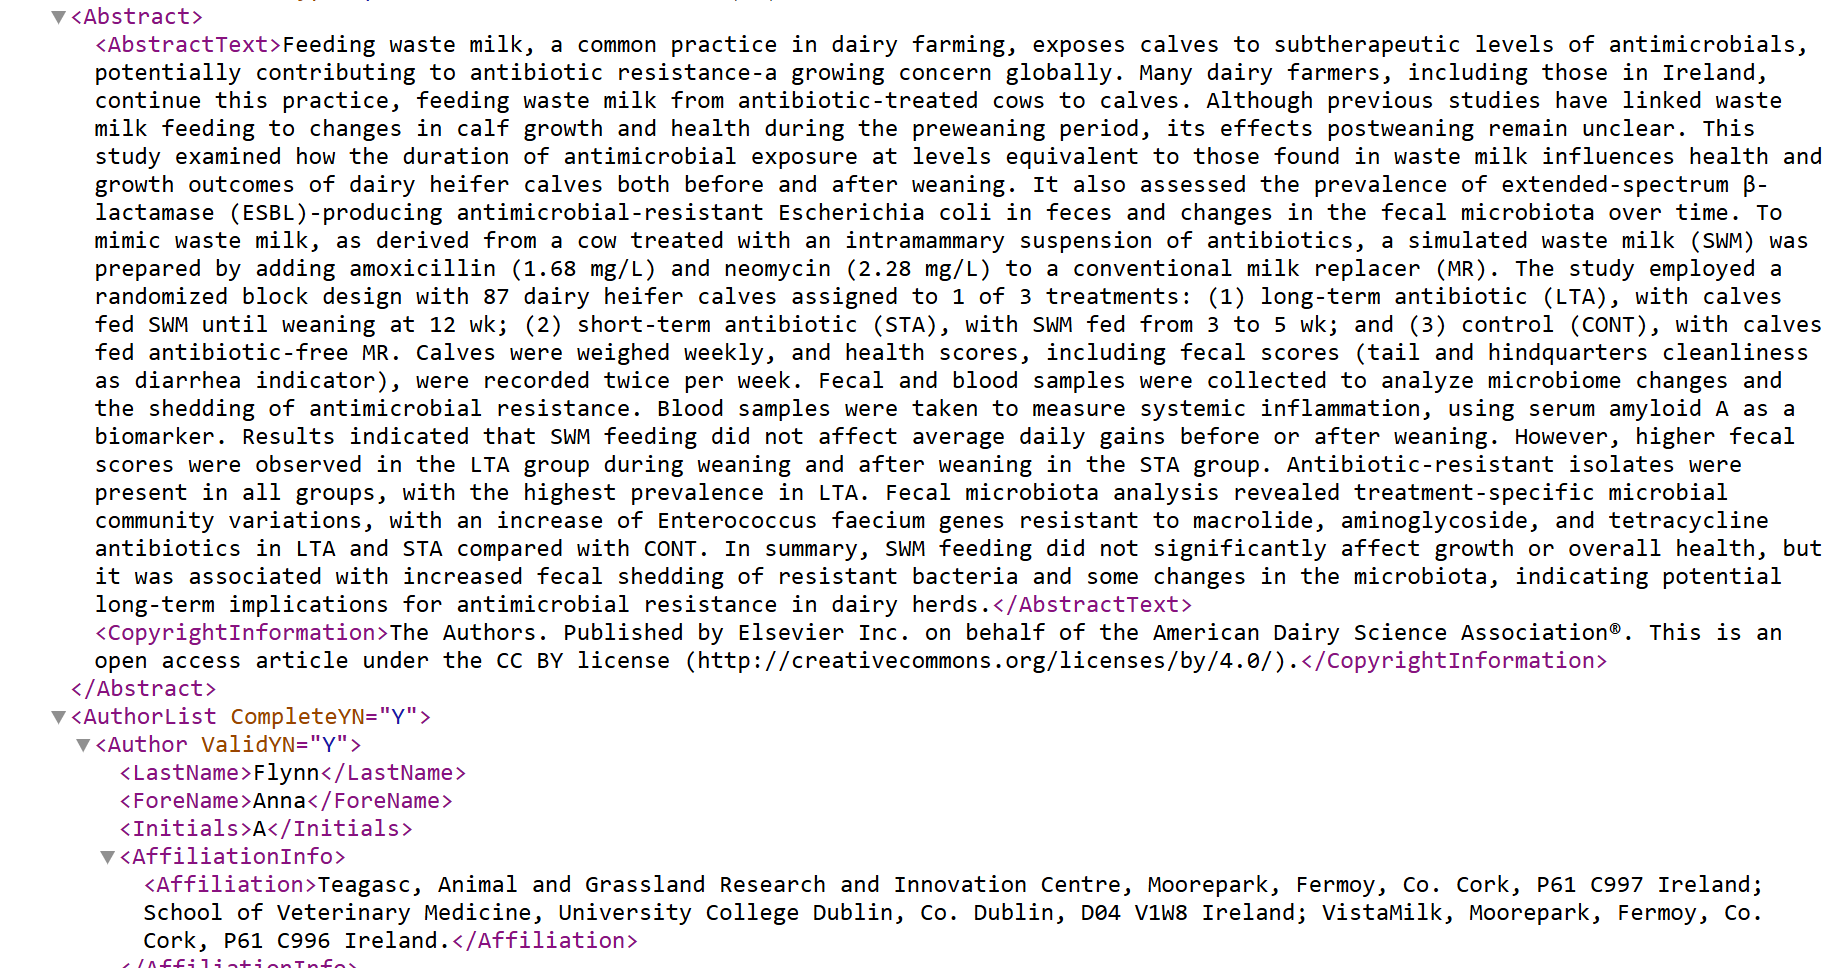
\includegraphics[width=0.95\linewidth, height=0.8\textheight, keepaspectratio]{imagens/art_pubmed1.png}
\caption{Artigo retornado pela API. Fonte: \cite{PubMed}}
\label{fig:art_pubmed}
\end{figure}


\begin{table}[H]
    \centering
    \resizebox{\textwidth}{!}{
        \begin{tabular}{c|p{2.5cm}|p{2.5cm}|p{3.5cm}|p{5cm}|p{3.5cm}}
             PubMedID & URL & JOURNAL & Title & Abstract & Keywords \\
             \midrule
             40383390 & \url{https://eutils.ncbi.nlm.nih.gov/entrez/eutils/efetch.fcgi?api_key={apikey}&db=pubmed&rettype=abstract&id=40383390} & Journal of Dairy Science & Effects of feeding a simulated waste milk on growth, health, fecal microbiota, and antibiotic resistance in dairy heifer calves. & Feeding waste milk, a common practice in dairy farming, exposes calves to subtherapeutic levels of antimicrobials, potentially contributing to antibiotic resistance... &
             antibiotic, average daily gain, microbiota, waste milk
        \end{tabular}
    }
    \caption{Exemplo de registro de artigo em CSV.}
    \label{tab:exemplo_art_csv}
\end{table}

No caso do livro de referência, após a conversão do PDF para texto, aplicaram-se regras de segmentação para identificar automaticamente o padrão das perguntas, exemplificado pela Imagem \ref{fig:ex_pergunta_livro}, geralmente numeradas e finalizadas por ponto de interrogação, e associá-las às respectivas respostas. Essa estrutura foi então exportada para CSV, tornando os dados mais acessíveis e consistentes para as etapas de avaliação e transformado  na Tabela \ref{tab:exemplo_livro_csv}.


\begin{figure}[H]
    \centering
    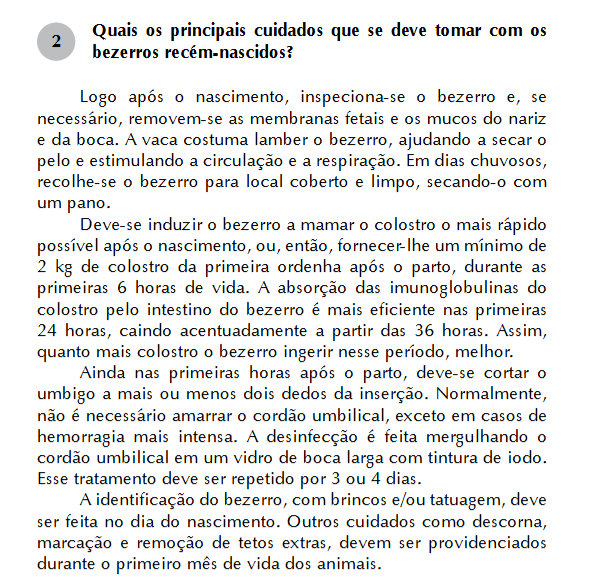
\includegraphics[width=0.60\linewidth]{imagens/ex_pergunta_livro.png}
    \caption{Exemplo de Pergunta: Fonte : \cite{embrapa2012gadoleite}}
    \label{fig:ex_pergunta_livro}
\end{figure}


\begin{table}[H]
    \centering
    \begin{tabularx}{\textwidth}{c|p{6cm}|>{\raggedright\arraybackslash}X}
        \textbf{Número} & \textbf{Pergunta} & \textbf{Resposta} \\
        \midrule
        2 & Quais os principais cuidados que se deve tomar com os bezerros recém-nascidos? & 
        Logo após o nascimento, inspeciona-se o bezerro e, se necessário, removem-se as membranas fetais e os mucos do nariz e da boca. A vaca costuma lamber o bezerro, ajudando a secar o pelo e estimulando a circulação e a respiração. Em dias chuvosos, recolhe-se o bezerro para local coberto e limpo, secando-o com um pano. Deve-se induzir o bezerro a mamar o colostro o mais rápido possível após o nascimento, ou, então, fornecer-lhe um mínimo de... \\
    \end{tabularx}
    \caption{Exemplo da coleta de Perguntas e Respostas do livro "500 Perguntas e Respostas sobre Gado de Leite" em CSV.}
    \label{tab:exemplo_livro_csv}
\end{table}



Esse processo contribuiu para uma maior eficácia e consistência dos dados, os quais serão utilizados na formulação das respostas pelos modelos, uma vez que essas informações influenciam diretamente o desempenho dos algoritmos na etapa de aprendizado.

\section{Mineração de Dados}
A etapa de Mineração de Dados teve como objetivo analisar e comparar o desempenho das estratégias de geração de respostas no domínio da pecuária leiteira. Inicialmente, foi utilizada a configuração com prompts \textit{Zero-shot} como linha de base. Posteriormente, essa abordagem foi comparada a sistemas baseados em RAG, alimentados com documentos específicos da área leiteira. O propósito foi verificar se há diferença significativa na qualidade das respostas geradas, avaliando em que medida a incorporação de informações contextuais contribui para o aprimoramento da geração no domínio estudado.

\subsection{Zero-shot}

O \textit{Zero-shot}, conforme descrito por \cite{zero-shot}, também é conhecido como instrução de tarefa. Ele consiste em formular um prompt que forneça uma descrição formal e detalhada da tarefa a ser realizada. Na Figura \ref{fig:Representação Zero-shot}, apresentamos o prompt utilizado neste projeto.

O \textit{Zero-shot} foi aplicado em duas APIs de modelos de linguagem: 

\begin{itemize}
    \item \textbf{API GPT (OpenAI)} \cite{openai2023chatgpt}: Disponibiliza modelos como GPT-3 e GPT-4, capazes de gerar respostas complexas e coerentes a partir de prompts detalhados.
    \item \textbf{API LLAMA (GroqAPI)} \cite{touvron2023llamaopenefficientfoundation}: Oferece modelos LLM gratuitos, como LLAMA-3.1, LLAMA-3.3 e LLAMA-8b, focados em tarefas de linguagem com boa performance para instruções específicas.
\end{itemize}

\begin{figure}[H]
    \centering
    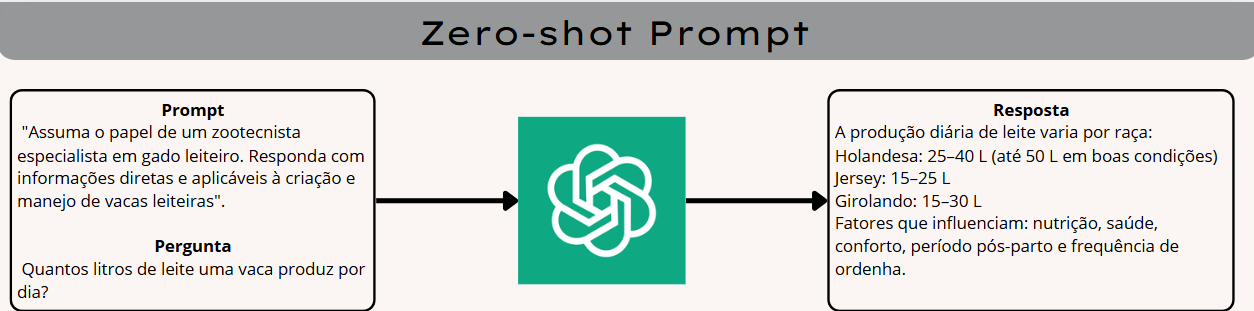
\includegraphics[width=1.0\linewidth]{imagens/zeroshot.png}
    \caption{Exemplo de Zero-shot. Fonte: Elaboração Própria}
    \label{fig:Representação Zero-shot}
\end{figure}

Como ilustrado na Figura \ref{fig:Representação Zero-shot}, o prompt define a tarefa a ser realizada e, junto da pergunta do usuário, é enviado ao modelo. Com base nesse contexto, o modelo gera a resposta mais adequada à tarefa, sem receber exemplos prévios.

    
\subsection{\textit{Few-shot}}

O \textit{Few-shot} difere do Zero-shot ao fornecer algumas demonstrações da tarefa durante a inferência, servindo como condicionamento para que o modelo execute a tarefa sem necessidade de atualização de pesos \cite{brown2020languagemodelsfewshotlearners}. Dessa forma, utiliza-se os exemplos fornecidos para que o modelo aprenda os padrões e estruture a resposta de forma adequada.

Essa estratégia apresenta algumas vantagens, como o aproveitamento de modelos pré-treinados e a fácil adaptação a novas tarefas. Entretanto, também possui desvantagens: requer, mesmo que em pequena quantidade, dados específicos para definir a tarefa e, geralmente, apresenta resultados inferiores aos de modelos ajustados por RAG, que utilizam informações do documento para contextualizar a resposta, resultando em uma resposta mais completa e fonte de dados verificável.

\begin{figure}[H]
\centering
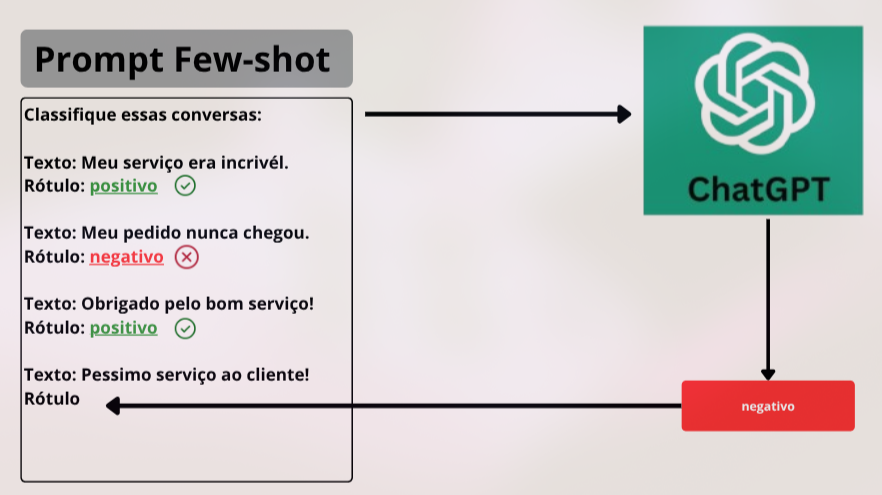
\includegraphics[width=0.75\linewidth]{imagens/few_shot1.png}
\caption{Representação adaptada e traduzida do Few-shot. Fonte: \cite{few-shotPromptImage}}
\label{fig:Representação Few-shot}
\end{figure}

A Figura \ref{fig:Representação Few-shot} demonstra o uso do \textit{Few-shot} na tarefa de classificar conversas quanto ao teor positivo ou negativo. Para isso, são fornecidos três exemplos de conversas acompanhados de suas classificações esperadas. Em seguida, apresenta-se um novo texto para que o modelo aplique a mesma tarefa. Com base no contexto fornecido pelos exemplos, o modelo analisa o texto em busca de padrões que permitam identificar a classe à qual ele pertence.

No presente trabalho, o Few-shot foi empregado como recurso complementar na construção dos prompts das abordagens baseadas em RAG, não sendo avaliado de forma isolada.

\subsection{RAG}

    O RAG é uma técnica que busca aprimorar a geração de respostas de modelos de LLM por meio do fornecimento de uma base de dados externa, como apontado por \cite{lewis2021retrievalaugmentedgenerationknowledgeintensivenlp}, a qual demonstra que esses modelos possuem limitações em tarefas que exigem conhecimento específico, atualizado ou explicações detalhadas.

    Nesse contexto, o RAG surge como uma solução para essas limitações, permitindo o uso de conhecimento proprietário. Documentos e artigos que não podem ser compartilhados publicamente, como e-mails, documentos internos e relatórios, podem ser utilizados como dados para a geração de respostas, proporcionando um contexto específico sobre o funcionamento da instituição, onde será aplicado. Além disso, o modelo pode citar fontes reais e atuais, mostrando de forma transparente a origem das informações utilizadas na geração da resposta, aumentando a veracidade dos dados e facilitando a verificação dos fatos pelo usuário.


\begin{figure}[H]
    \centering
    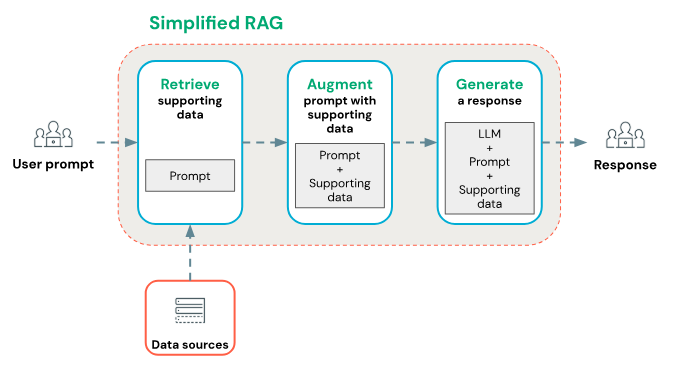
\includegraphics[width=0.8\linewidth]{imagens/representacao_rag.png}
    \caption{Representação do Funcionamento do RAG Fonte: \cite{microsoftRAG} }
    \label{fig:Representação RAG}
\end{figure}

Como descrito na Figura \ref{fig:Representação RAG}, o \textit{prompt} do usuário passa por três etapas, cada uma responsável por uma operação específica. A primeira etapa é a Recuperação, que analisa o \textit{prompt} e realiza a busca na base de dados externa, retornando informações de suporte que serão usadas como contexto adicional. Em seguida, ocorre a etapa de Aumentação, que combina os dados de suporte com o \textit{prompt} do usuário, gerando um \textit{prompt} mais contextualizado e relevante. Por fim, o \textit{prompt} aumentado é enviado ao modelo, permitindo a geração de respostas mais detalhadas e precisas, alinhadas com os dados de suporte.



Com isso foi estudamos 2 ferramentas que permitem realizar a tarefa de RAG:



\subsection{LightRAG}
LightRAG é um novo framework para aprimoramento de modelos de LLM por meio de RAG. Proposto por \cite{LightRag}, ele busca suprir duas principais limitações presentes nos sistemas de RAG tradicionais. A primeira delas é que muitos métodos dependem de representações planas, o que restringe a capacidade de compreender e recuperar informações baseadas nas relações entre entidades. A segunda limitação refere-se à lacuna de contexto, frequentemente insuficiente para manter a coerência entre diversas entidades, o que pode resultar em respostas que não atendem plenamente à consulta do usuário.

Para superar esses desafios, o LightRAG adota uma estratégia de recuperação em dois níveis, aprimorando a capacidade de compreensão e recuperação de informações tanto no nível inferior, voltado para a precisão e o detalhamento de entidades e seus relacionamentos, enquando o no nível superior, que abrange temas mais amplos e favorece a descoberta de conhecimento de forma contextualizada.

Além disso, o LightRAG incorpora estruturas de grafos no processo de indexação e recuperação de informações. A representação por meio de grafos facilita a modelagem eficaz das inter-relações entre entidades, permitindo uma recuperação de informação mais precisa e contextualizada.


Com essas abordagens, os autores alcançam maior efetividade e eficiência no sistema de RAG ao resolver três pontos cruciais, a Recuperação de Informação Compreensiva, garantindo a coleta completa do contexto e das interdependências entre entidades ao longo dos documentos. Posteriormente, a melhora na eficiência de recuperação, por meio da exploração da estrutura de conhecimento em grafos, o que reduz significativamente o tempo de resposta. Por ultimo a rápida adaptação a novos dados, permitindo que o sistema se ajuste rapidamente a atualizações, mantendo sua relevância em ambientes dinâmicos.

\subsubsection{Geração de Grafico}

\begin{figure}[H]
    \centering
    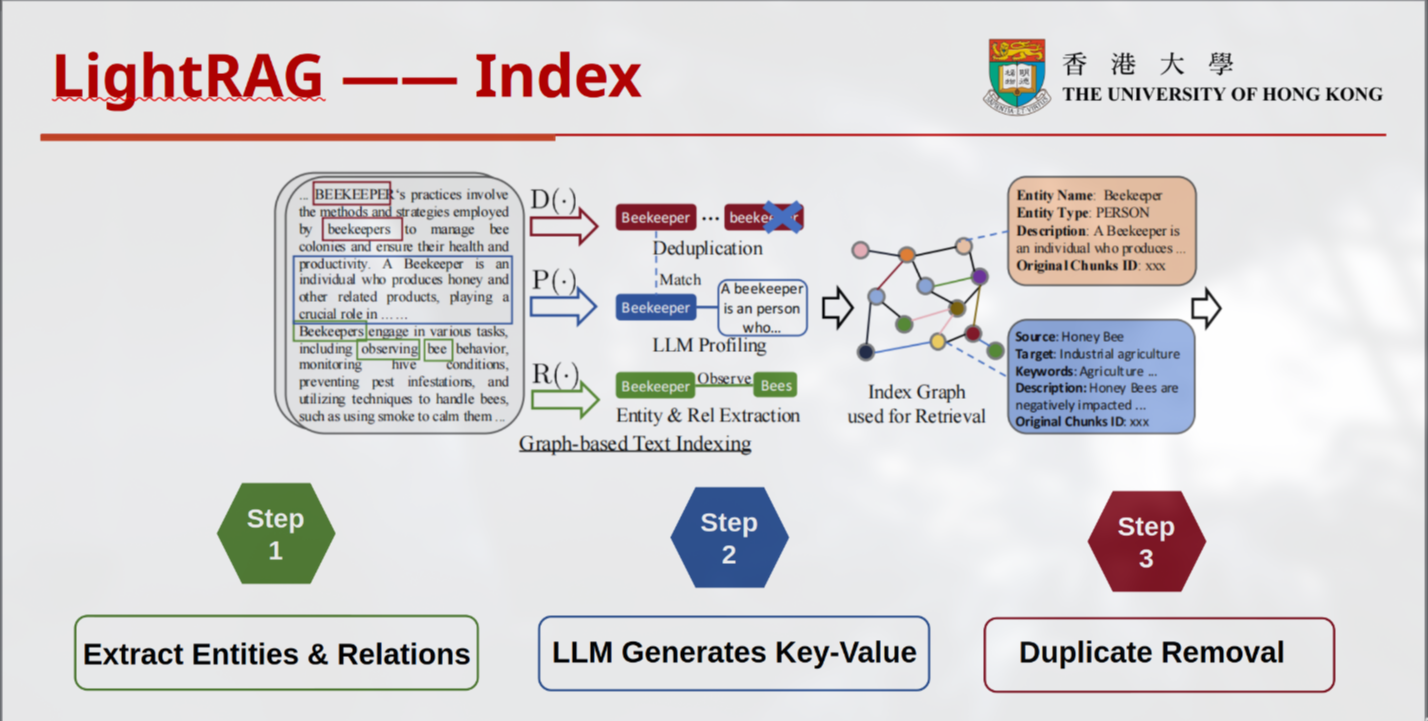
\includegraphics[width=1.0\linewidth]{image.png}
    \caption{Representação da Etapa de Indexação das informações no formato de gráfico. Fonte: \cite{LightRag}}
    \label{fig:light_rag_representation}
\end{figure}


A Figura \ref{fig:light_rag_representation} ilustra o fluxo de indexação e recuperação de conhecimentos no sistema. Inicialmente, documentos e dados brutos atravessam um pipeline dedicado à extração de entidades para a criação de nós e arestas para a criação e expansão do gráfico de conhecimento. Os nós armazenam as descrições das entidades, enquanto as arestas representam as relações semânticas com as demais entidades do gráfico, permitindo uma busca baseada na similaridade com a consulta do usuário.

O cálculo que representa a criação do Gráfo de conhecimento se dá pela formula \ref{eq:light_rag_graph_generation}

\begin{equation}
\label{eq:light_rag_graph_generation}
    \hat{D} = (\hat{V}, \hat{E}) = \text{Dedupe} \circ \text{Prof}(V, E), \quad \text{onde } V, E = \bigcup_{D_i \in D} \text{Recog}(D_i)
\end{equation}

Onde:
\begin{itemize}
    \item \( \hat{D}\): Grafo de Conhecimento;
    \item \( \hat{V}\):  Vértices do Grafo de Conhecimento;
    \item \( \hat{Ê}\): Arestas do Gráfo de Conhecimento;
    \item \(D \): Refêrente ao corpo do texto (Banco de Dados externo);
    \item \(D_i \): São as \textit{chunks} (segmentos) dos texto;
    \item \(Recog\): Função de Extração de Entidades e Relacionamentos;
    \item \(Prof\):  Função de Profilamento, usa um LLM para fazer a extração de chave-valor para a entidades e relacionamentos;
    \item \(Dedupe\): Função de Deduplicação, que faz a mesclagem de entidades repetidas;



\end{itemize}

Neste processo, cada função desempenha um papel específico. A primeira delas é o Recon (Reconhecimento), responsável pela extração de entidades e relacionamentos a partir de segmentos de texto. Utilizando um LLM, esta função analisa cada segmento isoladamente. Posteriormente, os resultados obtidos de todos os segmentos são unificados. Viabilizando a geração de um grafo de conhecimento, onde as conexões representadas de forma estruturada.

A segunda etapa é o Prof (Profilamento), responsável pela criação de chaves para cada entidade e relacionamento, visando facilitar o processo de recuperação. Nesta fase, um LLM é aplicado sobre o conjunto de segmentos para gerar pares chave-valor: as chaves garantem uma recuperação eficiente, enquanto os valores contêm parágrafos que resumem os trechos relevantes.

Por fim, na terceira etapa, atua o Dedupe (Deduplicação), responsável por identificar e unificar entidades e relacionamentos duplicados extraídos de diferentes segmentos. Esta etapa é crucial para otimizar o grafo, reduzindo seu tamanho ao eliminar redundâncias, mantendo apenas informações únicas e consolidando dados complementares.




\begin{figure}[H]
    \centering
    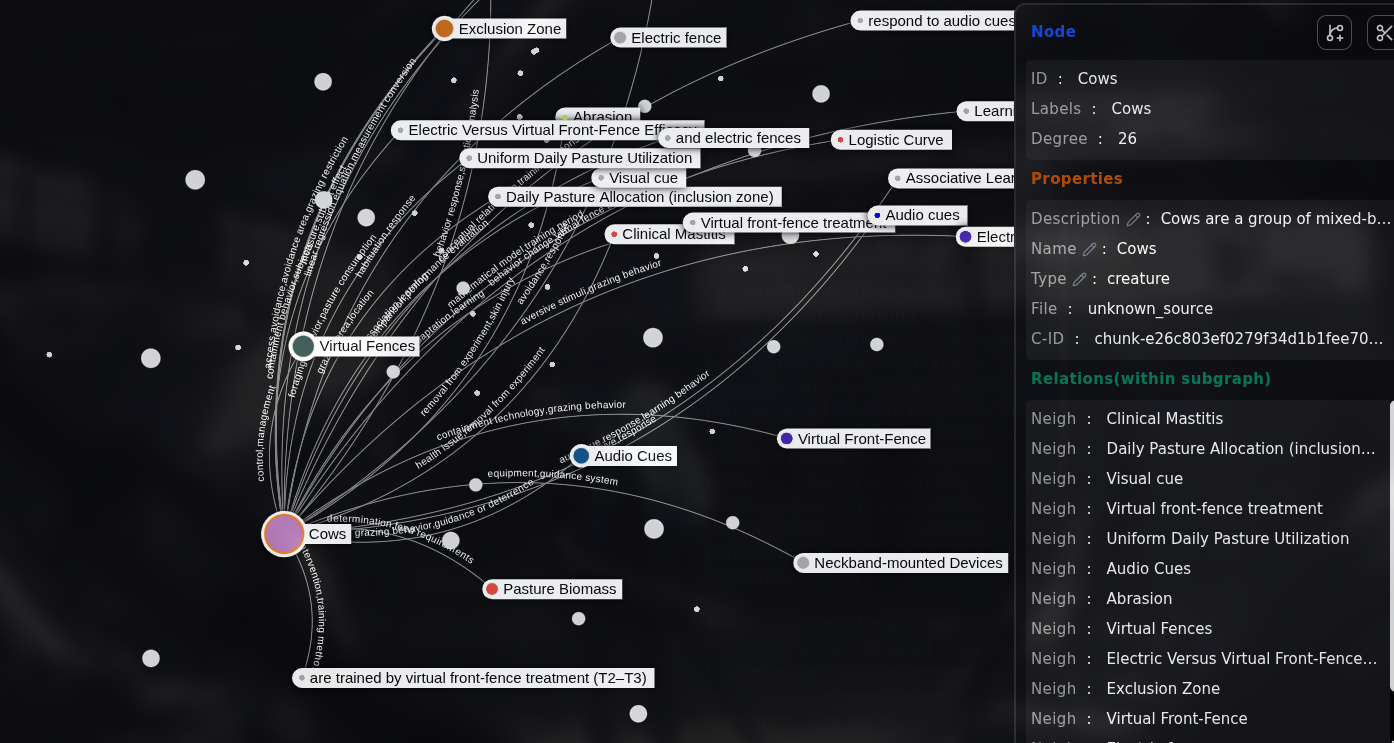
\includegraphics[width=1.0 \linewidth]{imagens/light_rag-representacao_grafo.png}
    \caption{Representação do Grafo de Conhecimento. Fonte: Elaboração Própria}
    \label{fig:light_rag-representacao_grafo}
\end{figure}

Finalizado o processo de indexação, obtém-se um Grafo de Conhecimento que consolida as propriedades das entidades descobertas, os documentos de origem e, fundamentalmente, as relações semânticas entre os elementos, como referenciado pela figura \ref{fig:light_rag-representacao_grafo}. A recuperação de informações ocorre por meio da navegação nesse grafo, onde a consulta do usuário é decomposta em conceitos de baixo nível \textit{(Low-Level Keys)} e conceitos abrangentes \textit{(High-Level Keys)}. O sistema realiza uma busca transversal em todos os nós correlacionados, retornando os trechos específicos de onde as informações foram extraídas. Esse fluxo fornece um contexto enriquecido e estruturado, permitindo que o modelo de linguagem gere respostas com maior precisão e fundamentação teórica.


\subsection{Geração de Resposta}

O processo de geração de resposta no sistema LightRAG inicia-se com a decomposição da consulta do usuário em dois níveis de granularidade: conceitos específicos e temas abrangentes. O prompt de instrução responsável por essa extração está representado na Figura \ref{fig:light_rag-prompt_extração de keywords}.


\begin{figure}[H]
    \centering
    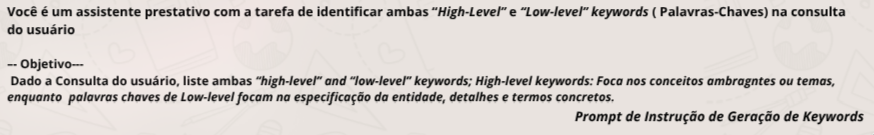
\includegraphics[width=1\linewidth]{imagens/light_rag-prompt_de_instrucao_extracao_de_keywords.png}
    \caption{Prompt de Instrução de Geração de Keywords. Fonte: Elaboração Própria}
    \label{fig:light_rag-prompt_extração de keywords}
\end{figure}

Para assegurar a consistência e o formato das saídas, utiliza-se a técnica de \textit{Few-shot}, cujo propósito é estabelecer um padrão de resposta esperado por meio da demonstração de exemplos práticos, conforme ilustrado na Figura \ref{fig:ligth_rag-prompt_geracao_de_entrada_de_keywords}.

\begin{figure}[H]
    \centering
    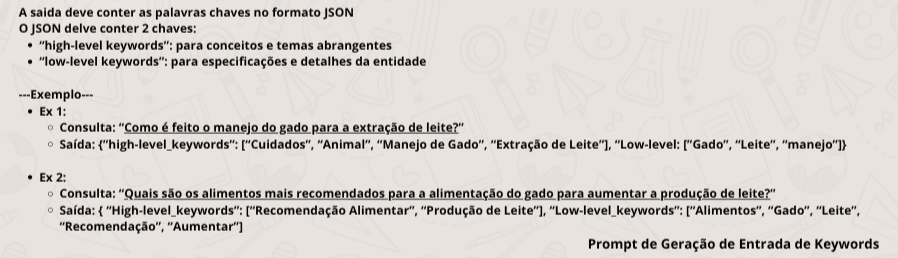
\includegraphics[width=1\linewidth]{ligth_rag-prompt_geracao_de_entrada_de_keywords.png}
    \caption{Prompt de Geração de Entrada de Keywords. Fonte: Elaboração Própria}
    \label{fig:ligth_rag-prompt_geracao_de_entrada_de_keywords}
\end{figure}


Uma vez extraídas as palavras-chave, o sistema realiza a navegação no grafo de conhecimento. A aplicação desse fluxo sobre a consulta original permite que o motor de busca identifique e recupere as entidades e relações mais relevantes, consolidando um contexto técnico enriquecido (Figura \ref{fig:light_rag-recuperacao_de_contexto}). Esse mecanismo mitiga a lacuna de contexto comum em sistemas tradicionais, resultando em uma resposta final mais completa e assertiva (Figura \ref{fig:light_rag-resposta_gerada}).

\begin{figure}[H]
    \centering
    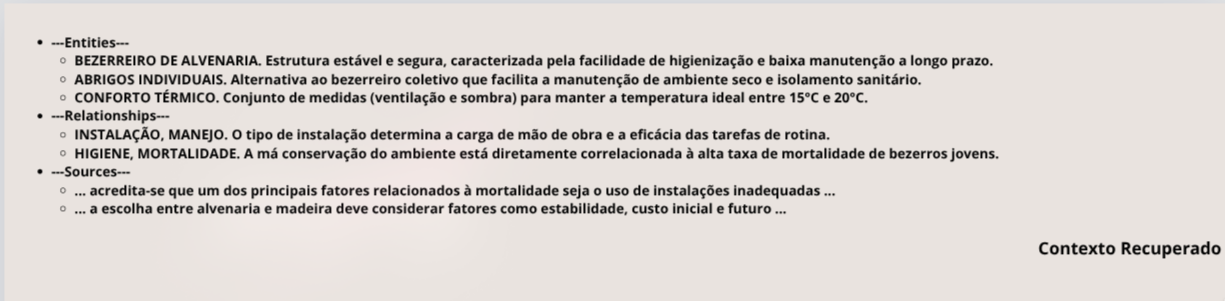
\includegraphics[width=1\linewidth]{imagens/light_rag-recuperacao_de_contexto.png}
    \caption{Contexto Recuperado pelo Ligth RAG. Fonte: Elaboração Própria}
    \label{fig:light_rag-recuperacao_de_contexto}
\end{figure}

\begin{figure}[H]
    \centering
    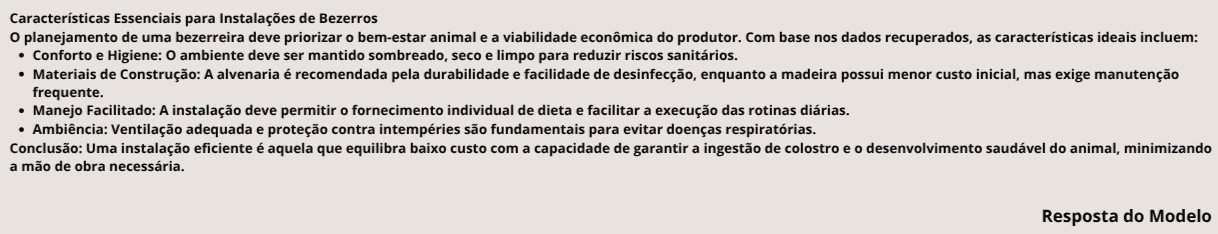
\includegraphics[width=1\linewidth]{imagens/light_rag-resposta_gerada1.png}
    \caption{Resposta Gerada pelo Ligth RAG. Fonte: Elaboração Própria}
    \label{fig:light_rag-resposta_gerada}
\end{figure}

\section{G-RAG-LiveRAG}
O G-RAG (ou LiveRAG) foi o sistema vencedor do desafio LiveRAG na conferência SIGIR 2025 (\textit{Special Interest Group on Information Retrieval}). A arquitetura propõe uma abordagem de Geração de Recuperação Aumentada baseada na criação de respostas hipotéticas para a consulta original do usuário. O objetivo central é o enriquecimento do vocabulário e do contexto semântico de perguntas que, rotineiramente, apresentam-se de forma excessivamente objetiva, como: "Qual vaca produz mais leite?".

Assim, o modelo gera uma resposta hípotetica imprecisas, como atribuir a maior produção à raça Jersey em vez da Holandesa, expandindo o vetor da consulta. Ao realizar a combinação da pergunta original com a resposta hipotética, o sistema amplia o argumento de busca, otimizando a relação semântica entre a consulta e os chunks de documentos indexados. Essa técnica eleva a taxa de recuperação de informações pertinentes, permitindo que a resposta final seja mais robusta e abranja conhecimentos que a pergunta simplista do usuário, isoladamente, não seria capaz de extrair da base de dados.

\subsection{Fluxo de Execução}

\begin{figure}[h]
    \centering
    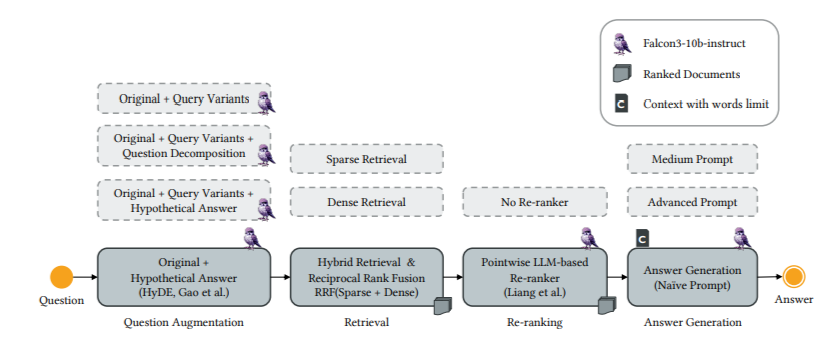
\includegraphics[width=1\linewidth]{imagens/fluxo_g_rag.png}
    \caption{Fluxo de geração de resposta do G-RAG, Fonte: \cite{G-RAG-LiveRAG}}
    \label{fig:g-rag-fluxo_de_trabalho}
\end{figure}

Ao passar a pergunta para o modelo, chega-se à primeira etapa do sistema, que consiste em aumentar a consulta original por meio de três técnicas possíveis, visando ampliar o contexto da dúvida do usuário e auxiliar o modelo a encontrar documentos que forneçam subsídios para uma resposta mais precisa. Esses documentos são selecionados com base na semelhança entre os termos presentes na resposta gerada e o conteúdo do acervo. Entre as estratégias disponíveis, destaca-se a Variação de Consultas \textit{(Query Variants)}, na qual definem-se $k$ variações da pergunta original para serem utilizadas como consultas de busca. Outra abordagem é a Consulta de Decomposição, que realiza diversas chamadas ao LLM para desmembrar a pergunta em subconsultas até identificar seu significado essencial, utilizando-o para reformular a questão original com detalhes mais importantes. Por fim, a Geração de Resposta Hipotética \textit{(Hypothetical Answer Generation)} permite que um modelo mais leve responda à pergunta inicial com maior flexibilidade. Embora essa resposta possa ser apenas parcialmente correta, ela cumpre o papel fundamental de servir como um contexto expandido de busca durante a etapa subsequente de recuperação.

Com a pergunta aumentada, passamos para a etapa de recuperação híbrida, composta por 2 tipos de recuperação,  a Esparsa, a qual busca por documentos que tenha a correspondencia exata das palavras chaves e entidades únicas contida na pergunta aumentada e a Recuperação Densa, faz a recuperação focada na semântica, retornando documentos que apresentem mesmas palavras ou significados semelhantes, utilizando a semelhança do cosseno para fazer essa comparação, dados todos os documentos recuperados, e aplicado o \textit{Reciprocal Rank Fusion} (RRF), para unir os 2 resultados obtidos por cada método é retorna apenas os documentos mais relevantes para a geração da resposta.

Com a lista de documentos relevantes para a pergunta partimos, passamos por um re ranqueamentos dos documentos obtidos na etapa anterior e passamos para um modelo de ponta avaliar, para verificar se os documentos contém informação necessária para responder a pergunta. Onde são rankeados pela taxa de semelhança, e caso a semelhança for inferior a 0.5, o documento e descartado. Posteriormente, para a geração da resposta final, passamos um prompt de instrução para o modelo descrevendo a tarefa a ser realizada pelo modelo, em conjunto dos documentos relevantes e o prompt aumentado, assim aprimorando a resposta gerada pelo modelo com prompt mais robusto e documentos relevantes.


\section{Avaliação do Modelo}
Para avaliar a qualidade das respostas geradas, foram utilizadas métricas amplamente difundidas na área de Processamento de Linguagem Natural, que comparam o texto de referência com o texto produzido pelo modelo. Além disso, foi aplicado o teste estatístico t-test como critério de desempate entre modelos que apresentaram resultados semelhantes. A função do t-test é verificar se a diferença entre as médias é estatisticamente significativa. Considerando um nível de significância de 5\%, quando o valor de \textbf{p} > 0{,}05, entende-se que não há diferença estatisticamente significativa entre os modelos; quando \textbf{p} < 0{,}05, pode-se assumir que há diferença significativa entre os desempenhos comparados. O teste foi aplicado considerando as médias das métricas obtidas em cada conjunto de respostas.



\subsection{BERTScore:}
O BERTScore é uma metrica de avaliação que busca fazer a comparação dado as sentenças de referência com uma sentença gerada, utilizando representações contextuais em forma de embeddings. A ideia central é calcular a taxa de correspondencia semantica entre os textos por meio da similidaridade do cosseno entre os vetores obtidos, como descrito por \cite{zhang2020bertscoreevaluatingtextgeneration}

\begin{figure}[H]
    \centering
    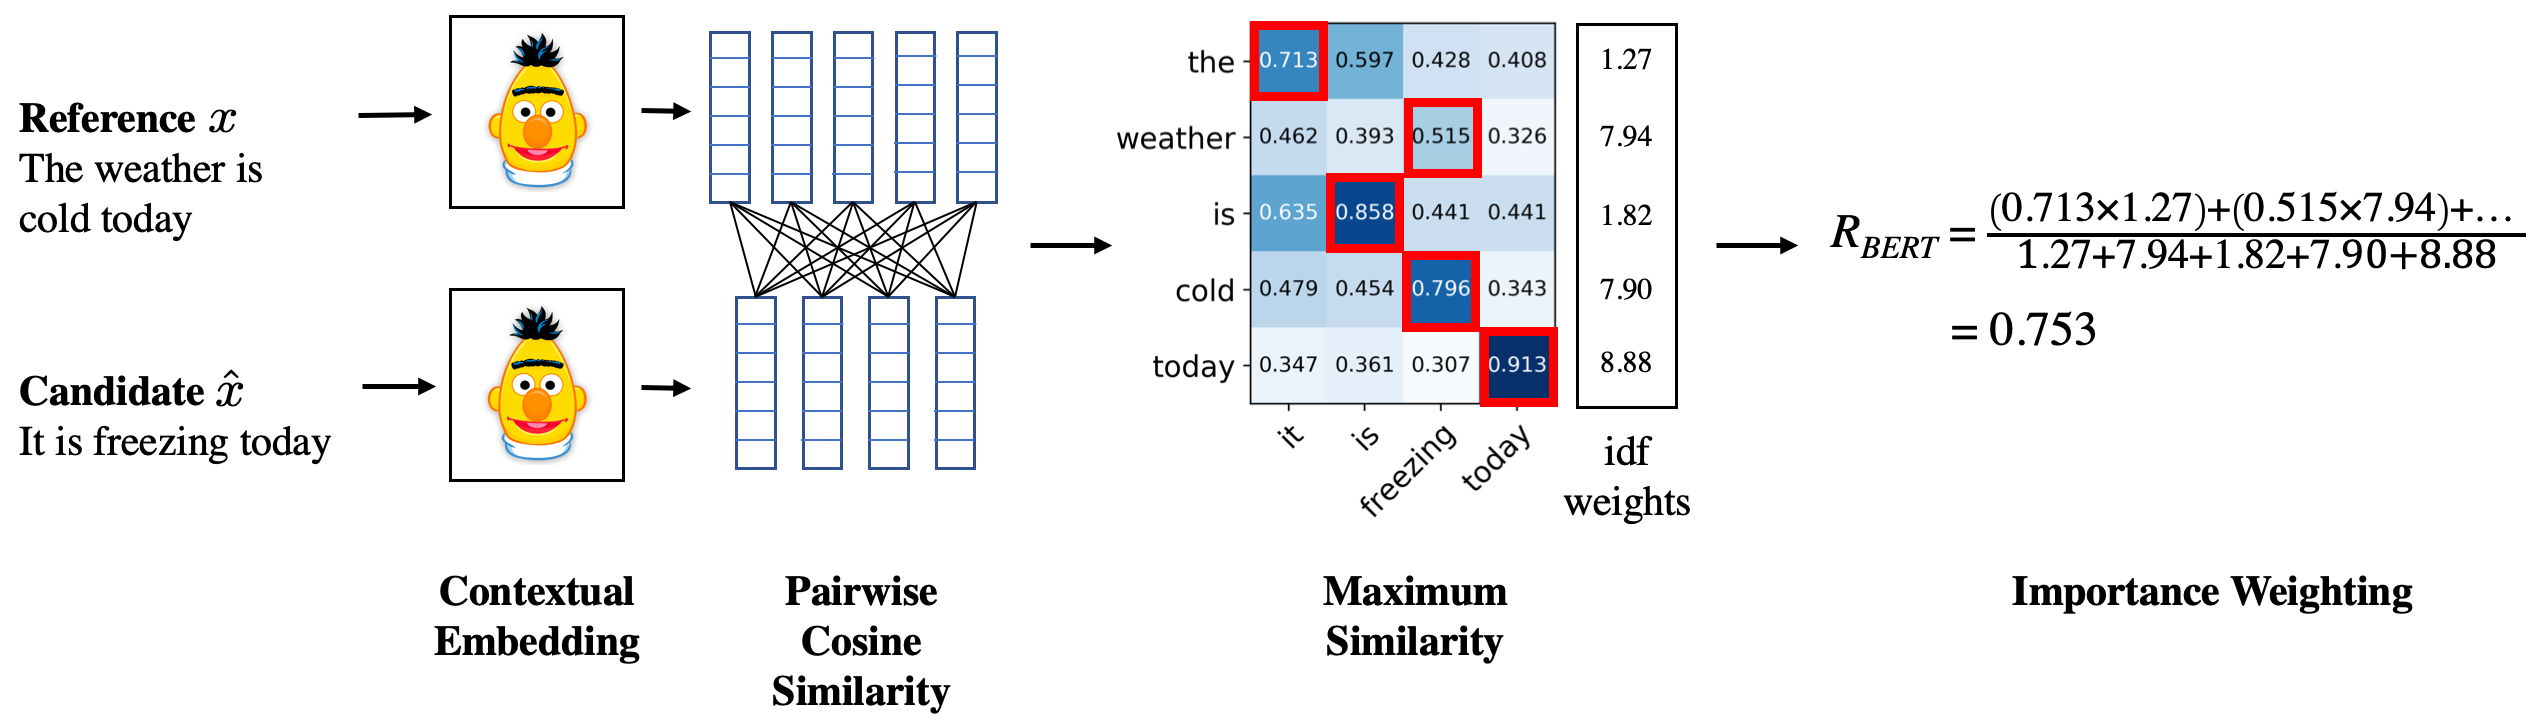
\includegraphics[width=0.8\linewidth]{imagens/bartscore.png}
    \caption{Ilustração do cálculo de recall $R_{BERT}$ Fonte:\cite{zhang2020bertscoreevaluatingtextgeneration}}
    \label{fig:bertscore_representation}
\end{figure}

O pipeline descrito na Figura \ref{fig:bertscore_representation} representa o processo executado pelo BERT, que consiste na conversão dos textos em vetores de embeddings contextuais, obtidos a partir das camadas do modelo BERT selecionado. Onde, posteriormente, é calculada a similaridade do cosseno, de modo a identificar as palavras que apresentam maior semelhança semântica entre os textos.


Possibilitando realizar a análise em ambos os sentidos: na precisão \ref{eq;precisonBert}, que mede o grau de correspondência semântica das palavras da sentença candidata em relação à referência e no recall \ref{eq;recallBert}, que avalia em que medida as palavras da referência encontram correspondência semântica na sentença candidata. Ao calcular a média harmônica entre os valores de precisão e recall \ref{eq;F1Bert}, obtém-se um equilíbrio entre as duas métricas, capturando de forma mais robusta a similaridade entre os textos.

\begin{equation}
\label{eq;precisonBert}
    P_{\text{BERT}} = \frac{1}{|y|} \sum_{y_j \in y} \max_{x_i \in x} (x_i^\top y_j)
\end{equation}

\begin{equation}
\label{eq;recallBert}
    R_{\text{BERT}} = \frac{1}{|x|} \sum_{x_i \in x} \max_{y_j \in y} (x_i^\top y_j)
\end{equation}

\begin{equation}
\label{eq;F1Bert}
    F_{BERT} = 2 \frac{P_{BERT} * R_{BERT}}{P_{BERT} + R_{BERT}}
\end{equation}


Onde:
\begin{itemize}
    \item \(x\): Conjunto de Embeddings das palavras do Texto Gerado.
    \item \(y\):  Conjunto de Embeddings das palavras do Texto Referência
    \item \(x_iT y_j\): Similaridade do Cosseno entre os embeddings do token candidato \(x_i\) e o embeddings do token de referência \(y_j\).
\end{itemize}

\subsubsection*{Exemplo do BERTScore}

Considere a sentença de referência:

\begin{itemize}
    \item \textbf{Referência}: \textit{``A vaca produz de 15 a 30 litros de leite todos os dias.''}
\end{itemize}

E duas sentenças geradas:

\begin{itemize}
    \item \textbf{Texto Gerado 1}: \textit{``A vaca dá entre 15 e 30 litros de leite diariamente.''}
    \item \textbf{Texto Gerado 2}: \textit{``A vaca come muito capim todos os dias.''}
\end{itemize}

O BERTScore converte cada palavra em representações vetoriais contextuais (embeddings) e calcula a similaridade do cosseno entre as palavras da referência e as da sentença candidata. Dessa forma, é possível capturar semelhanças semânticas mesmo quando há variações lexicais. 

A Tabela \ref{tab:exemplo_bertscore} mostra valores ilustrativos de precisão, recall e F1 do BERTScore para os dois textos gerados:

\begin{table}[H]
    \centering
    \begin{tabular}{lccc}
        \toprule
        \textbf{Sentença} & \textbf{Precisão ($P_{BERT}$)} & \textbf{Recall ($R_{BERT}$)} & \textbf{F1 ($F_{BERT}$)} \\
        \midrule
        Texto Gerado 1 & 0.94 & 0.93 & 0.935 \\
        Texto Gerado 2 & 0.41 & 0.39 & 0.40 \\
        \bottomrule
    \end{tabular}
    \caption{Exemplo de cálculo do BERTScore para duas sentenças geradas.}
    \label{tab:exemplo_bertscore}
\end{table}

Observa-se que o \textbf{Texto Gerado 1} obteve uma pontuação elevada, indicando alta similaridade semântica com a referência, mesmo utilizando palavras diferentes (\textit{``produz''} $\approx$ \textit{``dá''}, \textit{``todos os dias''} $\approx$ \textit{``diariamente''}). Já o \textbf{Texto Gerado 2} obteve valores baixos, pois apesar de compartilhar o contexto de ``todos os dias'', não preserva a informação central sobre a produção de leite.


\subsection{BARTScore:}
BARTScore é uma metrica de avaliação de textos gerados por LLMs, diferentemente do BERTScore, essa métrica não faz uso da similidaridade vetorial, mas sim da similariedade logarítimica, de que dado um texto base, o modelo BART é capaz de repoduzir a mesma saída, apartir do texto de referência \cite{NEURIPS2021_e4d2b6e6}, seguindo a Equação \ref{eq:BartScore}.
\newline

\textbf{Fórmula do BARTScore:}
\begin{equation}
    \label{eq:BartScore}
    BARTScore(x, y) = \sum_{t=1}^{m} w_t \log p(y_t \mid y_{<t}, x,\theta)
\end{equation}

Onde:
\begin{itemize}
    \item \(m\): Tamanho da sequência de saída
    \item \(w_t\): Pesos atribuido a cada token
    \item \(y_t\): Token na posição de saída
    \item \(x\): Texto de entrada
    \item \(\theta\): Parâmetros do modelo BART utilzado

\end{itemize}


\textbf{Exemplo}:

\begin{table}[H]
\resizebox{\linewidth}{!}{%
\begin{tabular}{|c|c|c|}
\hline
Texto Referência & Texto Candidato  & BARTScore \\
\hline
A vaca produz de 15 a 30 litros de leite todos os dias & A produção de laticínios por vacas é de aproximadamente 15 a 30 litros por dia & -0.43\\
A alimentação é um fator que influência diretamente na saúde do animal & Como realizar o controle de moscas do meio rural & -4.02 \\

\hline

\end{tabular}
}
\caption{Exemplo do cálculo do BartScore}
\label{tab:exemploBart}
\end{table}

Na Tabela \ref{tab:exemploBart}, para textos que apresentam uma alta taxa de semelhança semântica, eles recebem scores altos (valores menos negativos) e para texto considerados diferentes, apresentam scores mais baixos (mais negativos), indicando uma baixa relação semântica entre eles. 



\subsection{GPTScore:}
Como descrito por \cite{fu2023gptscoreevaluatedesire}, a métrica GPTScore baseia-se na utilização de um modelo GPT para atribuir uma probabilidade à geração de textos de alta qualidade, considerando como parâmetros a descrição da tarefa e a definição dos aspectos de avaliação. Para isso, é construído um prompt contendo a tarefa, os critérios de avaliação definidos e o contexto de entrada. Dado esse prompt, o modelo calcula a probabilidade de gerar o texto fornecido. Uma alta probabilidade indica que o texto está alinhado com o que o LLM “esperaria gerar”, dado o contexto e a tarefa, refletindo, assim, sua qualidade semântica e coerência.


\textbf{Fórmula do GPTScore:}

\begin{equation}
    GPTScore(h | d, a, S) = \sum_{t=1}^{m}w_t log p(h_t|h_{<t}, T(d,a,S), \theta)
\end{equation}

Onde:
\begin{itemize}
    \item \(h = (h1, h2, ..., hn)\): Textos a serem avaliados;
    \item \(w_t\): Peso do token na posição t;
    \item \(d\): Descrição da Tarefa; 
    \item \(a\): Aspectos a ser avaliado;
    \item \(S\): Texto fonte ou referência;
    \item \(T(d,a,S)\): Template do prompt que define o protocolo de avaliação. 
\end{itemize}

\textbf{Exemplo}:

\textbf{Texto de Referência} (S): "Vacas leiteiras podem produzir entre 15 a 30 litros por dia, dependendo da alimentação e cuidados."

\textbf{Tarefa} (d): "Classifique se a sentença gerada preserva as mesmas informarções do texto de referência."

\textbf{Aspecto} (a): "Corretude factual."

\textbf{Texto Candidato}(h):
\begin{itemize}
    \item 1. "As vacas produzem de 15 a 30 litros de leite diariamente."
    \item 2. "Vacas podem produzir até 50 litros de leite por dia."
\end{itemize}

\begin{table}[H]
    \centering
    \begin{tabular}{c|c|c|c}
         Tokens de h1     &   h1(log p) &  Tokens de h2    &     h2(log p)    \\
         
         \midrule
         
         As             &   -0.05     &   Vacas       &     -0.03       \\
         Vacas          &   -0.04     &   podem       &     -0.02       \\
         produzem       &   -0.03     &   produzir    &     -0.10       \\
         de             &   -0.02     &   até         &     -0.05       \\
         15             &   -0.01     &   50          &     -0.15       \\
         a              &   -0.01     &   litros      &     -0.01       \\
         30             &   -0.01     &   de          &     -0.01       \\
         litros         &   -0.02     &   leite       &     -0.02       \\
         de             &   -0.01     &   por         &     -0.01       \\ 
         leite          &   -0.03     &   dia         &     -0.03       \\
         diariamente    &   -0.02     &    -          &       -         \\
    
         \bottomrule
         
         \textbf{Soma}  &   -0.25     &       -       &      -0.34     \\
    \end{tabular}
    \caption{Exemplo do Cálculo de GPTScore}
    \label{tab:exemploGPTScore}
\end{table}

A Tabela \ref{tab:exemploGPTScore} apresenta as probabilidades logarítmicas atribuídas a cada token, considerando a definição da tarefa e os aspectos avaliados. Valores menos negativos indicam maior coerência do texto gerado em relação ao contexto de referência. No exemplo, o texto \textbf{h1} obteve um GPTScore mais alto, por manter consistência semântica e respeitar as informações do texto de referência. Em contraste, o texto \textbf{h2} recebeu um score inferior, pois afirmou que “vacas produzem até 50 litros de leite”, divergindo da referência, que estabelece o intervalo de 15 a 30 litros. Essa diferença evidencia como o GPTScore consegue penalizar incoerências factuais nos textos gerados.




\subsection{BLEU:} 
A métrica BLEU (Bilingual Evaluation Understudy — Assistente de Avaliação Bilíngue) foi uma das primeiras métricas propostas para avaliação de similaridade textual, como descrito em \cite{papineni-etal-2002-bleu}. A tarefa primária da técnica é comparar os n-gramas do texto candidato com os n-gramas do texto de referência, realizando a contagem das correspondências entre eles. Quanto maior a taxa de correspondências, melhor é considerado o candidato de tradução. O cálculo da métrica é representado por \ref{eq:BleuScore}:
\newline

\textbf{Fórmula da Métrica BLEU}

\begin{equation}
\label{eq:BleuScore}
    \text{BLEU} = BP \cdot \exp\left( \sum_{n=1}^{N} w_n \cdot \log p_n \right)
\end{equation}




Onde:
\begin{itemize}
    \item \(BP\) é o \textit{Brevity Penalty}:
    \begin{equation}
        BP =
        \begin{cases}
          1, & \text{se } c > r, \\[6pt]
          e^{\left(\tfrac{1-r}{c}\right)}, & \text{se } c \leq r.
        \end{cases}
\end{equation}
    \item \(c\)  Comprimento do texto candidato 
    \item \(r\) Comprimento do texto referência
    \item \(N\) Número de N gramas considerados
    \item \(p_n\) é a precisão para os \(n\)-gramas
    \item \(w_n\) é o peso atribuído a cada \(n\)-grama (1/N).
\end{itemize}


\textbf{Exemplo}:
\begin{itemize}
    \item Referência: "A vaca produz leite todos os dias."
    \item Texto gerado: "Vaca produz leite diariamente."
\end{itemize}


\begin{equation}
    p_1 = \frac{3}{4} = 0{,}75, \quad p_2 = \frac{2}{3} \approx 0{,}67, \quad BP = e^{\frac{1-7}{4}} \approx 0{,}47
\end{equation}

\begin{equation}
\label{eq:blue_ex}
    \text{BLEU} = 0{,}47 \times \exp\left(0{,}5 \log 0{,}75 + 0{,}5 \log 0{,}67\right) \approx 0{,}33
\end{equation}

O resultado obtido no exemplo \ref{eq:blue_ex} foi de aproximadamente $0{,}33$ indicando que, apesar de existir alguma sobreposição de palavras e expressões entre a frase gerada e a referência, a similaridade lexical ainda é limitada. Isso ocorre porque o BLEU não reconhece variações semânticas como sinônimos ou mudanças de ordem das palavras. No exemplo, embora ``diariamente'' seja um equivalente semântico de ``todos os dias'', a métrica penaliza a ausência de correspondência exata nos $n$-gramas.



\subsection{ROUGE-N:} 
ROUGE (Recall-Oriented Understudy for Gisting Evaluation) é um conjunto de métricas para avaliação da qualidade dos resumos \cite{lin-2004-rouge}. O objetivo do ROUGE é medir quanto do conteúdo do texto de referência aparece no texto gerado. Ao contrário do BLEU, que foca em precisão, a qual é a quantidade dos n-gramas da referência está contido no texto gerado, o ROUGE enfatiza o recall. Assim, o ROUGE é mais tolerante a variação da ordem das palavras e foca em analisar a informação essencial por inteiro, ao invés de exigir as mesmas palavras exatas. Representado pela formula \ref{eq:Rouge}


\textbf{Fórmula de ROUGE-N}

\begin{equation}
\text{ROUGE-N} =
\frac{
    \sum_{S \in \text{ReferenceSummaries}} \sum_{gram_n \in S} \text{Count}_{\text{match}}(gram_n)
}{
    \sum_{S \in \text{ReferenceSummaries}} \sum_{gram_n \in S} \text{Count}(gram_n)
}
\label{eq:Rouge}
\end{equation}

Onde:
\begin{itemize}
    \item \(\textit{ReferenceSummaries}\):  Conjunto de textos de referência
    \item \(\textit{\(n-gram\)}\): Sequência de N palavras consecutivas.
    \item \(\textit{Count}\) \(\textit{gram\_n}\): Quantidade de palavras n-gramas no texto de referência.
    \item \(Count_match(gram_n)\): Quantidade de n-gramas que aparece tanto na referência quanto no texto candidado
\end{itemize}

\textbf{Exemplo:}

Considere os seguintes textos:

\begin{itemize}
    \item Texto referência: "A vaca produz leite todos os dias."
    \item Texto gerado: "Vaca produz leite diariamente."
\end{itemize}

Os unigramas da referência são: \{A, vaca, produz, leite, todos, os, dias\}

Os unigramas do texto gerado são: \{Vaca, produz, leite, diariamente\}

A contagem dos unigramas da hipótese que aparecem na referência é 3: \{vaca, produz, leite\}

O total de unigramas na referência é 7.

Logo, o ROUGE-1 (recall) é calculado como:

\[
\text{ROUGE-1} = \frac{3}{7} \approx 0{,}429
\]

Esse valor indica que cerca de 42,9\% dos unigramas do texto de referência foram recuperados no texto gerado.



        % \chapter{Resultados Preliminares}
        % Os resultados parciais foram obtidos a partir da avaliação da capacidade dos modelos em responder às questões extraídas do livro Gado de Leite \cite{embrapa2012gadoleite}. Para aumentar a precisão das respostas geradas, aplicou-se um aprimoramento de prompting na configuração Zero-shot. Em seguida, as respostas foram avaliadas segundo as métricas propostas, resultando nos valores apresentados a seguir.



Inicialmente, realizou-se uma análise comparativa entre diferentes modelos da família Llama para avaliar variações em seus desempenhos e identificar possíveis ganhos em versões otimizadas. Os modelos avaliados incluíram o Llama-3-8B, Llama-3.1-8B-Instant, Llama-3-70B e Llama-3.3-70B-Versatile. Os resultados das métricas obtidas estão consolidados na Tabela \ref{tab:metricas_modelos_llama}.


\begin{table}[h]
\centering

\resizebox{\textwidth}{!}{%
\begin{tabular}{lccccc}
\toprule
\textbf{Modelos} & \textbf{BERTSCORE} & \textbf{BARTSCORE} & \textbf{GPTSCORE} & \textbf{BLEU} & \textbf{ROUGE-1} \\
\midrule

LLAMA-3-8b             & 0.70 (0.03) &  -3.32 (0.38) & -1.34 (0.16) &0.26 (0,08)  & 0.27 (0.09) \\

LLAMA-3.1-8b-instant   & 0.70 (0.03) & -3.31 (0.40) & -1.45 (0.15)& 0.26 (0.08) & 0.27 (0.09) \\

LLAMA3-70b             & 0.70 (0.03) & - 3.28 (0.38) & -0.94 (2.22) & 
0.27 (0.08) &  0.29 (0.10) \\

LLAMA-3.3-70b-versatile   & 0.70 (0.03) & -3.23 (0.37) & -1.05 (2.30) & 0.27 (0.08) & 0.27 (0.10) \\

\bottomrule
\end{tabular}%
}
\caption{Comparação de métricas entre modelos LLAMA}
\label{tab:metricas_modelos_llama}
\end{table}

A partir da análise dos dados, observa-se que o Llama-3-8B e sua variante Instant (caracterizada pela janela de contexto ampliada de 128K) apresentaram desempenhos estatisticamente equivalentes na tarefa de resposta a perguntas em regime zero-shot. Nota-se que, nas cinco métricas propostas, os resultados mantiveram-se consistentes, com divergências mínimas apenas no GPTScore. Padrão semelhante foi observado na comparação entre o Llama-3-70B e o Llama-3-3-70B-Versatile, onde as métricas de casamento de padrões e similaridade semântica não indicaram superioridade expressiva de um modelo sobre o outro.

Diante da ausência de ganhos significativos nas versões variantes para o escopo desta tarefa, optou-se por prosseguir com as avaliações utilizando os modelos base, garantindo maior estabilidade e comparabilidade nas etapas subsequentes do trabalho.



\begin{table}[h]
\centering
\resizebox{\textwidth}{!}{%
\begin{tabular}{lccccc}
\toprule
\textbf{Modelos} & \textbf{BERTSCORE} & \textbf{BARTSCORE} & \textbf{GPTSCORE} & \textbf{BLEU} & \textbf{ROUGE-1} \\
\midrule
GPT-3.5 Turbo             & 0.70 (0.05) & -3.22 (0.35) & -0.66 (2.06) & 0.28 (0.12) & 0.30 (0.16) \\
GPT-4                     & 0.71 (0.04) & -3.21 (0.42) & -0.96 (2.28) & 0.30 (0.09) &  0.33 (0.09) \\


LLAMA-3.1-8b      & 0.70 (0.03) & -3.31 (0.40) & -1.34 (0.16) & 0.26 (0.08) & 0.27 (0.09) \\
LLAMA-3.1-70b   & 0.70 (0.03) & -3.23 (0.37) & -1.05 (2.30) & 0.27 (0.08) & 0.27 (0.10) \\

LIGHT RAG + LLAMA 3.1-8b & 0.66 (0.08) & - 3.44 (0.42) & -1.37 (0.24) & 0.09 (0.13) & 0.24 (0.10) \\
LIGHT RAG + GPT-OSS:20b & 0.69 (0.07) & -3.52 (0.42) & --- & 0.22 (0.09) & 0.26 (0.09) \\


G-RAG + LLAMA 3.1-8b & 0.65 (0.06) & -3.59 (0.41) & -1.58 (0.17) & 0.09 (0.11)  & 0.26 (0.09) \\
G-RAG + GPT-OSS:20b & 0.64 (0.12) & -3.61 (0.65) & -1.50 (0.24) & 0.0009 (0.11) & 0.19 (0.09) \\
G-RAG + GPT-4 & 0.64 (0.06) & -3.57 (0.57) & -1.36 (0.14) &  0.04 (0.11) & 0.11 (0.09)\\
\bottomrule
\end{tabular}%
}
\caption{Comparação de métricas entre modelos Base}
\label{tab:metricas_modelos}
\end{table}

Dado os resultados apresentados na Tabela \ref{tab:metricas_modelos}, o modelo GPT-4 obteve desempenho superior aos demais nas métricas de avaliação de similaridade semântica. No BERTScore, alcançou pontuação média de 0.71, enquanto no BARTScore apresentou valor de -3.21, evidenciando maior proximidade semântica com o texto de referência (uma vez que valores menos negativos indicam maior similaridade). Esses resultados mostram que o GPT-4 foi consistente em gerar respostas semanticamente próximas aos textos de referência analisados. 

Entretanto, ao considerar a métrica GPTScore — que avalia a coerência semântica da resposta em relação à tarefa e ao aspecto de avaliação definido —, o GPT-4 apresentou desempenho inferior aos demais modelos. Isso indica que, embora suas respostas sejam semanticamente similares, não se alinharam de forma satisfatória ao critério de correção factual adotado. Diferentemente de métricas como BERTScore e BARTScore, que medem apenas similaridade semântica entre textos, o GPTScore se baseia na aderência factual às respostas de referência, revelando limitações do GPT-4 nesse aspecto específico.

Nas métricas de similaridade léxica, o GPT-4 também se destacou: obteve 0.30 no BLEU e 0.33 no ROUGE-1. Apesar de os valores absolutos serem baixos, o modelo superou os demais, evidenciando maior sobreposição léxica entre a resposta gerada e o texto de referência, o que indica melhor desempenho relativo na tarefa.

Ainda assim, observa-se que os valores obtidos permanecem relativamente baixos. Isso demonstra que, na problemática proposta — avaliar se as respostas geradas mantêm o mesmo teor informativo da referência —, há espaço significativo para aprimoramento, reforçando a necessidade de adaptação por meio de técnicas como RAG.

\section{Exemplos}

Nesta seção são apresentadas algumas perguntas acompanhadas de suas respectivas respostas de referência, em comparação com as respostas geradas pelo modelo, conforme ilustrado na Tabela \ref{tab:exemplo_respostas}.

\begin{table}[H]
    \centering
    \resizebox{\textwidth}{!}{
        \begin{tabular}{p{3.5cm}|p{5cm}|p{5cm}}
             \textbf{Pergunta} & \textbf{Resposta de Referência} & \textbf{Resposta Gerada} \\
             \midrule
             É aconselhável ordenhar as vacas antes do parto? & Não. Porque o bezerro precisa mamar a maior quantidade possível de colostro logo após o nascimento, a fim de garantir a ingestão de quantidade suficiente de imunoglobulinas. & Excelente pergunta! Como zootecnista especialista em gado leiteiro, posso afirmar que ordenhar antes do parto, popularmente conhecido como "ordenha seca", é uma prática comum e recomendada em muitas fazendas leiteiras. \\
            \midrule
            É preciso tostar os grãos de soja antes de fornecê-los às vacas em lactação? & Não necessariamente. A tostagem da soja apresenta a vantagem de eliminar alguns fatores antinutricionais presentes no grão cru, como inibidores de proteases, ácido fítico e urease. & Sim, é recomendado tostar os grãos de soja antes de fornecê-los às vacas em lactação. O processo de tostagem ajuda a melhorar a digestibilidade e a disponibilidade de proteína da soja para os ruminantes. \\
            \midrule
            Deve-se experimentar vários touros em uma vaca que não pega cria? & Não. A melhor conduta é realizar um exame ginecológico minucioso da vaca. Além disso, se for portadora de alguma doença do aparelho reprodutivo, a vaca pode contaminar todos os touros que a cobrirem. & Sim, é uma prática comum em reprodução animal tentar diferentes touros em uma vaca que não pega cria, para identificar se o problema está relacionado à capacidade reprodutiva da vaca ou do touro.
        \end{tabular}
    }
    \caption{Exemplos de perguntas e respostas de referência em comparação com as respostas geradas pelo modelo.}
    \label{tab:exemplo_respostas}
\end{table}

A análise dos exemplos evidencia divergências críticas. No primeiro caso, o modelo recomenda a ordenha antes do parto, desconsiderando a importância do colostro para a imunidade do bezerro. No segundo, sugere categoricamente a tostagem da soja, embora essa prática não seja obrigatória. No terceiro, indica experimentar vários touros em uma vaca que não pega cria, enquanto a referência recomenda inicialmente um exame ginecológico.  

Essas diferenças demonstram que os modelos podem gerar respostas com aparência de autoridade, mas tecnicamente incorretas ou imprecisas, reforçando a necessidade de ajustes e adaptações para uso confiável no setor leiteiro.



\section{Aplicação do RAG}

\subsection{Light RAG}


\subsection{G-LIVE-RAG}
\subsubsection{V1 (Aprimoramento por Documentos)}


\subsubsection{V2 - Aprimoramento por Prompt (\textit{ZeroShot} + Documento)}
\subsubsection{V3 - Expansão por Prompt Personalizado + Base de Documentos}





    \chapter{Resultados Experimentais}
        


Os resultados obtidos a partir da avaliação da capacidade dos modelos em responder ás questões extraidas do livro " 500 Perguntas 500 Respostas - Gado de Leite " \cite{embrapa2012gadoleite}. Para aumentar a precisão das respostas geradas, aplicou-se o aprimoramento de prompting \textit{Zero-shot}.

Inicialmente, realizou uma análise dos modelos disponiveis para o estudo e analisar como cada um respondeu as perguntas. Onde os modelos disponiveis foram: GPT-3.5, GPT-4, GPT-OSS, LLAMA-3.1-8b,  LLAMA3.1-8b-instant. LLAMA-3-70b e LLAMA-3.3-70b-versatile. Contudo, ao comparar os resultados obtidos entre os modelos da fámilia LLAMA, recebemos os seguintes resutlados demostrado na tabela \ref{tab:metricas_modelos_llama}

\begin{table}[h]
\centering

\resizebox{\textwidth}{!}{%
\begin{tabular}{lccccc}
\toprule
\textbf{Modelos} & \textbf{BERTSCORE} & \textbf{BARTSCORE} & \textbf{GPTSCORE} & \textbf{BLEU} & \textbf{ROUGE-1} \\
\midrule

LLAMA-3-8b               & 0.70 (0.03) & -3.32 (0.38) & -1.34 (0.16) & 0.26 (0.08)  & 0.27 (0.09) \\

LLAMA-3.1-8b-instant     & 0.70 (0.03) & -3.31 (0.40) & -1.45 (0.15) & 0.26 (0.08) & 0.27 (0.09) \\

LLAMA3-70b               & 0.70 (0.03) & -3.28 (0.38) & -0.94 (2.22) & 0.27 (0.08) &  0.29 (0.10) \\

LLAMA-3.3-70b-versatile  & 0.70 (0.03) & -3.23 (0.37) & -1.05 (2.30) & 0.27 (0.08) & 0.27 (0.10) \\

\bottomrule

\end{tabular}}
\caption{Comparação de métricas entre modelos LLAMA}
\label{tab:metricas_modelos_llama}
\end{table}

Ao verificar as diferenças entre os modelos LLAMA-3-8b e LLAMA-3.1-8b-instant, a que mais se destaca é o tamanho da janela de contexto, isto é, na quantidade máxima de informações que o modelo consegue processar em uma operação. Enquanto, o LLAMA-3-8b tem tamanho de 8K e a versão \textit{instant} é de 128K, o mesmo acontence para o LLAMA-3-70B e LLAMA-3.3-70b-versatile. No caso de tentarem responder a mesma pergunta, percebe que os valores de sua métrica são muito similares, o qual resultou na remoção dos modelos com maior janela de contexto, devido não terem apresentado um ganho significativo para essa tarefa.

Assim, os principais modelos selecionados foram: GPT-3.5-Turbo, GPT-4, GPT-OSS:20b LLAMA-3:8b e LLAMA-3:70b. Os resultados das métricas obtidas estão consolidados na Tabela \ref{tab:metricas_modelos}.

\begin{table}[H]
\centering

\resizebox{\textwidth}{!}{%
\begin{tabular}{lccccc}
\toprule
\textbf{Modelos} & \textbf{BERTSCORE} & \textbf{BARTSCORE} & \textbf{GPTSCORE} & \textbf{BLEU} & \textbf{ROUGE-1} \\
\midrule
   
    ZERO SHOT + GPT-4             & \textbf{0.71 (0.04)} & \textbf{-3.21 (0.42)} & -1.45 (0.15) & \textbf{0.30 (0.09)} &  \textbf{0.33 (0.09)} \\
    ZERO SHOT + GPT-3.5 Turbo     & 0.70 (0.05) & -3.22 (0.35) & \textbf{-1.36 (0.14)} & 0.28 (0.12) & 0.30 (0.16) \\
    ZERO SHOT + GPT-OSS :20b      & 0.68 (0.03) & -3.39 (0.31) & -1.58 (0.36) & 0.158 (0.05) &  0.15 (0.08) \\
    ZERO SHOT + LLAMA-3:8b        & 0.70 (0.03) & -3.31 (0.40) & -1.34 (0.16) & 0.26 (0.08) & 0.27 (0.09) \\
    ZERO SHOT + LLAMA-3:70b       & 0.70 (0.03) & -3.23 (0.37) & -0.94 (2.22) & 0.27 (0.08) & 0.27 (0.10) \\

    LIGHT RAG + GPT-OSS:20b       & 0.69 (0.07) & -3.52 (0.42) & -1.54 (0.13) & 0.22 (0.09) & 0.26 (0.09) \\
    LIGHT RAG + LLAMA-3:8b       & 0.66 (0.08) & -3.44 (0.42) & -1.37 (0.24) & 0.09 (0.13) & 0.24 (0.10) \\

    G-LIVE-RAG + GPT-4            & 0.65 (0.06) & -3.57 (0.57) & -1.36 (0.14) & 0.04 (0.11) & 0.11 (0.09) \\
    G-LIVE-RAG + LLAMA-3:8b      & 0.65 (0.06) & -3.59 (0.41) & -1.58 (0.17) & 0.09 (0.11) & 0.26 (0.09) \\
    G-LIVE-RAG + GPT-OSS:20b      & 0.64 (0.12) & -3.61 (0.65) & -1.50 (0.24) & 0.00 (0.11) & 0.19 (0.09) \\
    

\bottomrule
\end{tabular}}
\caption{Comparação de métricas entre modelos Base}
\label{tab:metricas_modelos}
\end{table}


A Tabela \ref{tab:metricas_modelos} apresenta os valores médios obtidos em cada métrica, juntamente com seus respectivos desvios padrão, permitindo observar o desempenho de cada modelo em diferentes aspectos da qualidade textual das respostas geradas.

Com o objetivo de sintetizar o desempenho geral considerando simultaneamente todas as métricas avaliadas, foi elaborado um ranqueamento baseado na média da posição obtida por cada modelo. Inicialmente, cada modelo recebeu uma posição em cada métrica analisada. Em seguida, foi calculada a média dessas posições, permitindo identificar quais modelos apresentaram melhor desempenho global.

O resultado desse procedimento é apresentado na Tabela \ref{tab:rank_models}.
\begin{table}[H]
\centering

\begin{tabular}{lcc}
\toprule
\textbf{Posição} & \textbf{Modelos} & \textbf{Média Geral} \\
\midrule
   
     1º     &   ZERO SHOT + GPT-4             & 2.00   \\
     1º     &   ZERO SHOT + GPT-3.5 Turbo     & 2.00   \\
     3º     &   ZERO SHOT + LLAMA-3-70b       & 2.40   \\
     4º     &   ZERO SHOT + LLAMA-3.1-8b      & 3.20   \\
     
     5º     &   LIGHT RAG + GPT-OSS:20b       & 5.60   \\

     6º     &   ZERO SHOT + GPT-OSS:20b       & 6.00   \\
     7º     &   LIGHT RAG + LLAMA-3:8b        & 6.20   \\
    
     8º     &   G-LIVE-RAG + GPT-4            & 6.60   \\
     9º     &   G-LIVE-RAG + LLAMA3.1 8b      & 7.00   \\
    10º     &   G-LIVE-RAG + GPT-OSS:20b      & 7.80   \\

\bottomrule
\end{tabular}
\caption{Ranqueamento entre os modelos}
\label{tab:rank_models}
\end{table}

A partir da média das posições obtidas nas métricas avaliadas, foi possível identificar os modelos com melhor desempenho geral. Observa-se que as configurações \textit{Zero-shot + GPT-4} e \textit{Zero-shot + GPT-3.5 Turbo} apresentaram as melhores médias de ranking, indicando resultados muito próximos entre si nas métricas analisadas.

Dado os resultados apresentados na Tabela \ref{tab:metricas_modelos} e na Tabela \ref{tab:rank_models}, o modelo GPT-4 obteve desempenho superior na maioria das métricas de avaliação de similaridade semântica em relação aos outros modelos base com aplicação de \textit{Zero-shot}. No BERTScore, alcançou pontuação média de 0.71, enquanto no BARTScore apresentou valor de -3.21, evidenciando maior proximidade semântica com o texto de referência, uma vez que valores menos negativos indicam maior similaridade. Esses resultados mostram que o GPT-4 foi consistente em gerar respostas semanticamente próximas aos textos de referência analisados. 

Entretanto, ao considerar a métrica GPTScore, o qual avalia a coerência semântica da resposta em relação à tarefa e ao aspecto de avaliação definido, o GPT-4 apresentou desempenho inferior aos demais modelos. Isso indica que, embora suas respostas sejam semanticamente similares, não se alinharam de forma satisfatória ao critério de correção factual adotado. Diferentemente de métricas como BERTScore e BARTScore, que medem apenas similaridade semântica entre textos, o GPTScore se baseia na aderência factual às respostas de referência, revelando limitações do GPT-4 nesse aspecto específico.

Nas métricas de similaridade léxica, o GPT-4 também se destacou: obteve 0.30 no BLEU e 0.33 no ROUGE. Apesar de os valores absolutos serem baixos, o modelo superou os demais, evidenciando maior sobreposição léxica entre a resposta gerada e o texto de referência, o que indica melhor desempenho relativo na tarefa.

Ainda assim, observa-se que os valores obtidos permanecem relativamente baixos. Isso demonstra que, na problemática proposta de avaliar se as respostas geradas mantêm o mesmo teor informativo da referência, há espaço significativo para aprimoramento, reforçando a necessidade de adaptação por meio de técnicas como RAG.



% ====
 % Explicação do RAG:
% =======

A análise isolada das métricas quantitativas na tabela \ref{tab:metricas_modelos} sugere uma redução de desempenho nas arquiteturas de RAG em comparação ao modelo base com aplicação do \textit{Zero-shot}. No entanto, uma avaliação qualitativa e manual das saídas revela um cenário distinto. Ao contrastarmos as respostas para a questão de exemplo usada a seguir, podemos observar os comportamentos divergentes que justificam a oscilação dos índices automáticos, conforme detalhado na Tabela \ref{tab:exemplo_respostas}.

\begin{itemize}
    \item{Exemplo}: Quais as características de uma boa instalação para bezerros?
    
    \item{Resposta Ouro}: Deve ser de baixo custo, oferecer conforto para os animais e facilitar o manejo. Acredita-se que um dos principais fatores relacionados à alta taxa de mortalidade de bezerros jovens seja o uso de instalações inadequadas. E certos tipos de instalação exigem muita mão de obra, dificultando a execução das tarefas de rotina. É importante salientar que há a opção de utilização de abrigos individuais, que estão substituindo o bezerreiro, principalmente, pela facilidade de manutenção de ambiente sombreado, seco e limpo, e pela possibilidade de ser mudado de local. Além disso, permite o fornecimento individual de leite, volumoso, concentrado e água.
\end{itemize}

Resposta Geradas para a pergunta:
\begin{table}[H]
    \centering

    \resizebox{\textwidth}{!}{%
        \begin{tabular}{p{4cm} | p{12cm}} % Definido o tamanho para evitar erros de renderização
            \toprule
            \textbf{Modelo} & \textbf{Resposta Gerada} \\
            \midrule
            
            \textbf{ZERO SHOT + LLAMA 3:70b} & Excelente pergunta! Uma boa instalação para bezerros é fundamental para o desenvolvimento saudável e rápido dos animais. Aqui estão as características essenciais: \begin{itemize} \item \textbf{Localização:} Área segura e protegida; \item \textbf{Espaço:} Densidade de 2,5 a 3 $m^2$ por animal; \item \textbf{Ventilação:} Altura mínima de 3m entre chão e teto; \item \textbf{Iluminação:} Natural e complementar (florescentes); \item \textbf{Climatização:} Sistema de aquecimento e resfriamento (15°C a 20°C). \end{itemize} \\
            
            \midrule
            
            \textbf{LIGHT RAG + LLAMA 3:70b} & A escolha entre um bezerreiro de alvenaria e um de madeira deve considerar fatores como estabilidade e custo. \\ & \textbf{Alvenaria:} Alta estabilidade, fácil limpeza (pode ser lavada) e baixa manutenção. \\ & \textbf{Madeira:} Custo de construção baixo, mas manutenção cara e frequente, com dificuldade de higienização por absorver umidade. \\
            
            \midrule
            
            \textbf{G-LiveRAG + LLAMA 3:70b} & Uma boa instalação deve garantir visibilidade, espaço para movimentação e manutenção rigorosa da higiene. \newline \newline \textit{Nota do Modelo:} No entanto, a pergunta não está diretamente relacionada aos documentos fornecidos (focados em análise de Colostro Bovino). O modelo utilizou conhecimento prévio para responder. \\
            
            \bottomrule
        \end{tabular}
        }
            \caption{Exemplos de perguntas e respostas de referência em comparação com as respostas geradas pelos modelos.}
    \label{tab:exemplo_respostas}
\end{table}


O modelo \textit{Zero-Shot} + LLAMA-3:70B gera uma resposta baseada estritamente em seu conhecimento prévio, aquirido durante o seu treinamento. Embora estruturada, a resposta apresenta a falta de especificidade técnica voltada à realidade da pecuária bovina, listando itens que podem ser considerados excessivos ou de difícil implementação prática para o manejo sugerido pelo referencial da Embrapa.

Em contrapartida, o LightRAG + LLAMA-3:70B demonstra uma transição para um caráter consultivo na geração dessa resposta. A resposta é direcionada à resolução do problema, oferecendo opções de materiais e avaliando fatores como orçamento e facilidade de higienização. Esta abordagem aproxima-se da utilidade esperada de um assistente especializado, mesmo que a divergência vocabular em relação à "Resposta Ouro" penalize as métricas de similaridade léxica.

Quanto ao G-LiveRAG + LLAMA-3:70B, observa o impacto positivo da técnica de aprimoramento de prompt. O sistema conseguiu expandir a consulta original, gerando uma resposta com estrutura similar à de referência. Contudo, o sistema explicitou uma limitação crítica: a ausência de informações pertinentes no corpus documental fornecido. Os documentos indexados, com foco na análise química de colostro bovino, não continham o contexto necessário sobre instalações físicas.

Este achado é determinante para a interpretação dos resultados: a eficácia de um sistema RAG é estritamente limitada pela relevância e abrangência da sua base de dados. A inferioridade das métricas de RAG em relação ao modelo base com \textit{Zero-shot} não decorre de uma falha na arquitetura, mas de uma "lacuna informacional" entre as perguntas do livro de referência e o conteúdo técnico dos artigos científicos selecionados \cite{GONTIJO2025101097}. Consequentemente, o modelo acaba por recorrer ao seu conhecimento interno, enquanto o processo de recuperação de documentos não relacionados introduz ruídos que reduzem a precisão semântica calculada pelas métricas automáticas.

\section{Impacto da Engenharia de Prompt}
A qualidade da consulta enviada ao recuperador é um fator determinante para a eficácia do sistema G-LiveRAG. Prompts com baixo contexto frequentemente resultam em recuperações imprecisas, uma vez que a consulta original pode carecer de termos técnicos presentes nos documentos de domínio. A técnica de aprimoramento busca mitigar essa lacuna através da reformulação da consulta e do direcionamento da instrução do sistema.

O G-LiveRAG utiliza instruções específicas para balizar a geração, focando em respostas objetivas fundamentadas nos documentos fornecidos. Essa abordagem visa aumentar a confiabilidade do sistema ao permitir a checagem de veracidade dos fatos. Os níveis de complexidade de instrução avaliados são:

\begin{itemize}
    \item{Simples}: Um \textit{prompt} simples que define uma persona para o modelo e define que a resposta deve  ser baseadas nos documentos recuperados.
    
    \item{Médio}: Esse \textit{Prompt} é mais restritivo, onde limita a resposta apenas ao conteúdo dos documentos, caso não tenha contexto suficiente para responder retorna "Eu não sei".
    
    \item{Avançado}: Mais restritivo que o \textit{prompt} anterior, agora o modelo está mais limitado, sendo proibido de agregar qualquer conhecimento externo ou inferir qualquer detalhe dado o contexto retornado e tem que prover uma resposta mais conscisa seguindo a pergunta realizada e as informações extraidas dos documentos.
    
    \item{Customizado}: A versão customizada une a versatilidade do prompt Simples ao definir uma persona especializada no domínio da pecuária leiteira, com o rigor do prompt Avançado. Ele estabelece uma hierarquia de fontes onde o contexto recuperado é a prioridade absoluta, mas permite a expansão técnica baseada em conhecimento científico consolidado caso os documentos sejam insuficientes, desde que essa distinção seja explicitamente sinalizada na resposta.
\end{itemize} 


 Os prompt utilizados estão detalhados na Tabela \ref{tab:g_live_rag_prompts_instrucao}.

\begin{table}[H]
\centering

\resizebox{\textwidth}{!}{%
\begin{tabular}{l p{14cm}} % p{} permite quebra de linha automática
\toprule
\textbf{Variações de Prompt} & \textbf{Prompt de Instrução (JSON Structure)} \\
\midrule

Simples & \texttt{\{ "system\_prompt": "You are a helpful assistant. Answer the question based on the provided documents.", "primary\_prompt": "Documents: \textbackslash n\textbackslash n\{context\}\textbackslash n\textbackslash nQuestion: \{question\}\textbackslash n\textbackslash nAnswer: " \}} \\ 

\midrule

Médio & \texttt{\{ "system\_prompt": "You are given a question and you MUST respond by EXTRACTING the answer from provided documents. If none of the documents contain the answer, respond with *'I don't know'*.", "primary\_prompt": "Documents:\textbackslash n\textbackslash n\{context\}\textbackslash n\textbackslash n*Question: \{question\}* \textbackslash n Answer: " \}} \\ 

\midrule

Avançado & \texttt{\{ "system\_prompt": "You must respond based strictly on the information in provided passages. Do not incorporate any external knowledge or infer any details beyond what is given in the passages.", "primary\_prompt": "Provide a concise answer to the following question based on the information in the provided documents. Documents:\textbackslash n\textbackslash n\{context\}\textbackslash n\textbackslash n*Question: \{question\}*\textbackslash nAnswer: " \}} \\ 

\midrule

Customizado & \texttt{\{ "system\_prompt": "Você é um Consultor Sênior em Pecuária Leiteira. Sua abordagem combina a análise rigorosa dos documentos fornecidos com o conhecimento científico consolidado da zootecnia. Seu objetivo é fornecer a resposta mais completa e prática possível. Se os documentos forem insuficientes, você deve expandir a explicação usando sua base de conhecimento, sinalizando quando estiver trazendo boas práticas externas ao texto.", "primary\_prompt": "Utilize o contexto em \{context\} como base principal para responder à pergunta: \{question\}. ### Instruções de Composição: 1. \textbf{Prioridade de Contexto:} Inicie a resposta utilizando os dados e recomendações presentes nos documentos fornecidos. 2. \textbf{Expansão Técnica:} Caso os documentos não cubram todos os aspectos da pergunta, utilize seus conhecimentos em manejo, nutrição e sanidade animal para complementar a resposta. 3. \textbf{Clareza de Fontes:} Diferencie o que é recomendação direta dos documentos e o que é prática geral da zootecnia. 4. \textbf{Formatação:} Organize a explicação de forma técnica e clara. Resposta Consultiva:" \}} \\

\bottomrule
\end{tabular}
}
\caption{Definição de Variações de Prompts de Instrução por Nível de Complexidade}
\label{tab:g_live_rag_prompts_instrucao}
\end{table}


Conforme observado, as variações Médio e Avançado possuem um caráter estritamente restritivo. Elas limitam a resposta ao contexto extraído, inibindo o uso do conhecimento prévio (\textit{parametric memory}) do modelo e substituindo possíveis incertezas pela cláusula de salvaguarda "Eu não sei". Embora essa rigidez reduza a taxa de alucinação, ela torna o sistema extremamente dependente da clareza da consulta e da riqueza da base de documentos. Caso haja ambiguidade em qualquer um desses pontos, a resposta tende a ser inconclusiva.

Os impactos dessas diferentes abordagens de instrução nas métricas de desempenho estão consolidados na Tabela \ref{tab:g_live_rag_metrica_aprimoramento_de_prompt}.

% TABELA COM A COMPARAÇÃO ENTRE OS RESULTADOS de NAIVE _ MEDIUM _ ADVANCED _ CUSTOM

\begin{table}[h]
\centering

\resizebox{\textwidth}{!}{%
\begin{tabular}{lccccc}
\toprule
\textbf{Prompt de Geração de Consulta} & \textbf{BERTSCORE} & \textbf{BARTSCORE} & \textbf{GPTSCORE} & \textbf{BLEU} & \textbf{ROUGE-1} \\
\midrule

Simples      & 0.65 (0.05) & -3.58 (0.41) & -1.85 (0.24) &  0.09 (0.11)     & 2.19E-01 (0.07) \\
Médio        & 0.33 (0.14) & -5.17 (0.84) & -2.04 (0.26) &  6.73E-78 (0.07) & 2.82E-02 (0.08) \\
Avançado     & 0.56 (0.12) & -3.87 (0.78) & -2.23 (0.35) &  2.71E-78 (0.06) & 0.11 (0.89) \\
Customizado  & 0.67 (0.03) & -3.59 (0.35) & -1.47 (0.11) &  0.18 (0.10)     & 0.24 (0.08)\\

\bottomrule
\end{tabular}}
\caption{Comparação de métricas em relação ao nivel de prompt de instrução}
\label{tab:g_live_rag_metrica_aprimoramento_de_prompt}
\end{table}


\subsection{Análise dos Resultados}
A análise dos dados revela que o nível Customizado obteve o melhor equilíbrio entre similaridade semântica e fidelidade léxica. Enquanto os níveis Médio e Avançado sofreram uma degradação severa nas métricas (com valores de BLEU e ROUGE-1 próximos a zero devido à recusa do modelo em responder na ausência de correspondência exata), o prompt Customizado agiu como um mecanismo de "compensação semântica".

Ao definir uma persona de consultor e permitir a expansão técnica baseada em conhecimento consolidado da zootecnia, o sistema contornou as limitações de uma base documental reduzida. Esse enriquecimento prova que, para modelos de menor escala, a flexibilização controlada da instrução, priorizando o contexto, mas permitindo a fundamentação técnica externa, é o caminho mais viável para manter a utilidade prática do sistema sem comprometer a autoridade do conteúdo.


    
		
	\chapter{Conclusão}
        Em resumo, a aplicação de técnicas de aprimoramento sobre modelos de LLM, como \textit{Zero-shot}, \textit{Few-shot} e RAG, mostraram-se caminhos relevantes para explorar aspectos capazes de melhorar a geração dos modelos. Isso ocorre ao definir um papel para tornar a resposta mais específica, através de uma persona de autoridade, ao estabelecer o padrão de resposta esperado, por meio de exemplos que definem a estrutura, e, por último, ao utilizar documentos do domínio do problema, como o de gado leiteiro, fazendo com que as respostas sejam baseadas em documentos que são referências no assunto, facilitando a confirmação de fatos.

Contudo, ao avaliar os resultados obtidos, o uso de \textit{Zero-shot} nos modelos de LLM mostrou-se uma técnica capaz de gerar respostas melhores em comparação às que tiveram a aplicação de sistemas RAG. Um grande fator que pode ter influenciado esse resultado inferior foi a quantidade limitada de documentos, delimitando as respostas apenas aos dados neles presentes e diminuindo sua eficácia. Adicionalmente, o avanço de modelos que implementam busca nativa, como as versões recentes do ChatGPT e Gemini, sugere que parte desses dados já possa estar integrada à base de conhecimento dos modelos. Outro fator que impactou nos resultados do RAG, especificamente no caso do \textit{Light RAG} foi a complexidade computacional para adicionar um novo documento ao sistema, como também a alta latência e custo por indexação, restringindo a avaliação a apenas 2 modelos e com um conjunto de dados bem limitado. Essas limitações indicam o ganho significativo de sistemas complexos de recuperação estão condicionadas a quantidade e qualidade da base de conhecimento fornecida e à viabilidade de recursos computacionais.

Com base nessas observações, como trabalhos futuros, sugere-se analisar como o uso de técnicas de ajuste fino (Fine-Tuning) pode impactar a geração de respostas em modelos treinados no domínio específico da pecuária leiteira, em comparação aos resultados obtidos com Zero-shot e sistemas de RAG, considerando as métricas utilizadas neste trabalho.

Além disso, sugere-se a utilização de uma maior quantidade de dados apurados por especialistas da área, como artigos, revistas e apresentações científicas sobre pecuária leiteira, avaliando o impacto que a quantidade de documentos exerce no resultado final das respostas geradas por um modelo base, a fim de identificar se a qualidade e a quantidade dos documentos coletados são relevantes para responder adequadamente às perguntas propostas.

O sistema desenvolvido neste trabalho está disponível publicamente para reprodução e extensão em: \url{https://gitlab.com/Zander404/TCCs_DairyColletor.git}
.



	% ----------------------------------------------------------
	% Capitulo com exemplos de comandos inseridos de arquivo externo 
	% ----------------------------------------------------------
	
	\include{abntex2-modelo-include-comandos}
	
	% ---
	% Finaliza a parte no bookmark do PDF
	% para que se inicie o bookmark na raiz
	% e adiciona espaço de parte no Sumário
	% ---
	\phantompart
	
	
	
	% ----------------------------------------------------------
	% ELEMENTOS PÓS-TEXTUAIS
	% ----------------------------------------------------------
	\postextual
	
	% ----------------------------------------------------------
	% Referências bibliográficas
	% ----------------------------------------------------------
	\bibliography{artigoTCC}
	
	% ----------------------------------------------------------
	% Glossário
	% ----------------------------------------------------------
	%
	% Consulte o manual da classe abntex2 para orientações sobre o glossário.
	%
	%\glossary
	
	
	%---------------------------------------------------------------------
	% INDICE REMISSIVO
	%---------------------------------------------------------------------
	
	\phantompart
	
	\printindex
	
	
\end{document}
